\documentclass[manuscript,nonacm,12pt,letterpaper]{acmart}

% Strip ACM publication boilerplate (reference format, copyright block,
% "Manuscript submitted to ACM" footer, DOI, contact-info footnote)
\settopmatter{printacmref=false, printccs=false, printfolios=true}
\setcopyright{none}
\renewcommand\footnotetextcopyrightpermission[1]{}
\acmDOI{}
\acmISBN{}
\usepackage[utf8]{inputenc}
\usepackage{amsmath}
\usepackage{amsfonts}
\usepackage{graphicx}
\usepackage{tabularx}
\usepackage{subcaption}
\usepackage{float}
\usepackage{physics}


\author{Anish Murthy}
\affiliation{\institution{DigiPen Institute of Technology, Redmond}}
\title{Simulating an Elastic Body as a Mass Spring System of Particles}
\begin{document}

\graphicspath{ {./images/} }

\begin{abstract}
This report presents the design and implementation of a three-dimensional elastic body using Lagrangian dynamics and a mass–spring–damper formulation. The system models an elastic solid as a cube of point masses connected by linear springs with viscous damping, allowing for deformation under external forces such as gravity and interaction with a rigid floor. The equations of motion are derived in two complementary ways: (i) Newtonian mechanics, by summing the spring, damping, and external forces on each particle and applying Newton’s second law, and (ii) Lagrangian dynamics, by defining the kinetic and potential energies for the multi-particle system and introducing damping via a Rayleigh dissipation function to obtain the Euler–Lagrange equations with dissipation. Both derivations lead to the same coupled system of second-order differential equations, which are integrated numerically using a momentum-based time-stepping scheme. To improve stability and demonstrate elastic behavior, selected particles are constrained as fixed anchor points. The simulation successfully demonstrates oscillatory motion, damping, deformation, and recovery behavior characteristic of elastic materials
\end{abstract}
\maketitle

% -------------------------------------------------
\section{Introduction}
\label{Sec1:Intro}
Physical simulation of deformable bodies is a fundamental problem in computer graphics, robotics, and computational physics. Unlike rigid bodies, deformable objects require modeling internal forces that resist stretching, compression, and shear. One common and computationally efficient approach is the mass–spring model, in which an object is simulated as point masses connected by springs that approximate elastic behavior.

This project implements a three-dimensional mass–spring–damper cube and derives its mechanics using both Newtonian and Lagrangian viewpoints. The Newtonian derivation begins from explicit force laws (Hooke’s law for springs and a velocity-proportional damping term) and applies Newton’s second law to each particle. The Lagrangian derivation begins from the energy definitions, which are the kinetic energy, the gravitational potential energy, and the elastic potential energy, and incorporates damping using a Rayleigh dissipation function. The presentation of both derivations serves two purposes: validates the force model used in the implementation and demonstrates the equivalence between the force-based and energy-based formulations for this system.

% -------------------------------------------------
\section{System Overview}
\label{Sec2:SysOverview}

\subsection{Discretized Elastic Body}
\label{Sec2.1:Body}

The elastic body is represented as a cubic lattice of $N$ point masses. Each particle $i$ has a position ${x}_i(t) \in \mathbb{R}^3$ and a mass $m_i$. Rotational degrees of freedom are not modeled; the system represents a deformable continuum rather than a rigid body.

Particles are connected to neighboring particles via linear springs. For interior particles, connections are made to all neighbors within a $3 \times 3 \times 3$ neighborhood, excluding the particle itself. This results in up to 26 springs per particle, including axis-aligned neighbors, face diagonals, and body diagonals. This connectivity provides resistance to stretching and shear deformation.

Two particles are designated as fixed anchor points. These particles are constrained to remain stationary throughout the simulation and serve to stabilize the system and demonstrate elastic deformation relative to fixed supports.

\subsection{Degrees of Freedom}
\label{Sec2.1:DegreesOfFreedom}

Each non-fixed particle has three translational degrees of freedom corresponding to its position components $(x_i, y_i, z_i)$. The simulation stores linear momentum $\mathbf{p}_i(t)$
for each particle, from which velocity is computed as
\[
\mathbf{v}_i = \frac{\mathbf{p}_i}{m_i}.
\]

% -------------------------------------------------
\section{System Parameters and Initial Conditions}
\label{Sec3:SysParams}

\subsection{Physical Parameters}
\label{Sec3.1:PhysicalParams}

The simulation uses the following parameters:
\begin{itemize}
    \item Particle mass:
    \[
    m_i = 1 \quad \text{for all particles}.
    \]
    \item Particle spacing (axis-aligned spacing):
    \[
    L_0 = 2.
    \]
    \item Spring Rest lengths:
    \begin{itemize}
        \item Axis-aligned neighbors: $2$
        \item Face diagonals: $2\sqrt{2}$
        \item Body diagonals: $2\sqrt{3}$
    \end{itemize}
    \item Spring stiffness and damping:
    \begin{itemize}
        \item Structural springs: $(k_s, c_s)$
        \item Diagonal springs: $(k_d, c_d)$, scaled relative to structural springs
    \end{itemize}
    \item Gravitational acceleration:
    \[
    g = 9.81.
    \]
    \item Time step:
    \[
    \Delta t = \frac{1}{60},
    \]
    with multiple substeps per frame for numerical stability.
\end{itemize}

\subsection{Initial Configuration}
\label{Sec3.1:InitialConfig}

Particles are initially placed in a regular cubic lattice such that all springs are at their rest lengths. This configuration corresponds to a stress-free equilibrium state. All particle momenta are initialized to zero:
\[
\mathbf{p}_i(0) = \mathbf{0}.
\]

Two particles located at selected corners of the cube are designated as fixed anchor points and remain stationary throughout the simulation.

\subsection{Boundary Conditions}
\label{Sec3.2:BoundaryConditions}

A rigid horizontal floor is introduced at a fixed height. Particle-floor interaction is enforced using a non-penetration constraint combined with a restitution-based collision response. After each integration step, if a particle is found to have penetrated the floor plane, its position is projected back onto the surface.

The normal component of the particle velocity is modified according to a coefficient of restitution $e = 0.3$, such that
\[
v_n^{+} = -e\, v_n^{-},
\]
where $v_n^{-}$ and $v_n^{+}$ denote the normal velocity components immediately before and after collision, respectively. This produces a partially elastic collision that allows particles to bounce while still dissipating energy. Tangential velocity components are left unchanged.

This simple boundary treatment provides a computationally efficient approximation of particle-floor interaction that is sufficient to demonstrate elastic deformation, bouncing, and settling behavior in the simulated elastic body.

% -------------------------------------------------
\section{Newtonian Formulation of the Equations of Motion}
\label{Sec4:Newtonian}

This section derives the governing dynamics using Newtonian mechanics. The deformable body is modeled as a set of point masses connected by springs and dampers. For each particle $i$, Newton's second law is applied in vector form:
\begin{equation}
m_i \ddot{\mathbf{x}}_i = \mathbf{F}_i^{\text{int}} + \mathbf{F}_i^{\text{ext}},
\label{eq:newton_2nd_law}
\end{equation}
where $\mathbf{x}_i(t) \in \mathbb{R}^3$ is the particle position, and the right-hand side consists of internal forces from springs/dampers and external forces such as gravity and contact.

\subsection{Spring Geometry and Notation}
\label{Sec4.1:SpringNotation}

Consider a spring connecting particles $i$ and $j$. Define
\begin{align}
\mathbf{d}_{ij} &= \mathbf{x}_i - \mathbf{x}_j, \\
L_{ij} &= \|\mathbf{d}_{ij}\|, \\
\hat{\mathbf{e}}_{ij} &= \frac{\mathbf{d}_{ij}}{L_{ij}},
\end{align}
where $L_{ij}$ is the current spring length and $\hat{\mathbf{e}}_{ij}$ is the unit direction vector pointing from particle $j$ to particle $i$. The spring has rest length $L_{0,ij}$, stiffness $k_{ij}$, and damping coefficient $c_{ij}$. Particle velocities are denoted $\mathbf{v}_i = \dot{\mathbf{x}}_i$ and $\mathbf{v}_j = \dot{\mathbf{x}}_j$.

\subsection{Elastic Spring Force (Hooke's Law)}
\label{Sec4.2:SpringForce}

The scalar extension (positive for tension, negative for compression) is
\begin{equation}
\Delta L_{ij} = L_{ij} - L_{0,ij}.
\end{equation}
A linear spring exerts a restoring force along the spring direction. The spring force applied to particle $i$ due to particle $j$ is
\begin{equation}
\mathbf{F}^{\text{spring}}_{ij \rightarrow i}
= -k_{ij} (L_{ij} - L_{0,ij}) \, \hat{\mathbf{e}}_{ij}.
\label{eq:newton_spring_force}
\end{equation}
By Newton's third law, the force on particle $j$ is equal and opposite:
\begin{equation}
\mathbf{F}^{\text{spring}}_{ij \rightarrow j}
= -\mathbf{F}^{\text{spring}}_{ij \rightarrow i}.
\end{equation}

\subsection{Viscous Damping Along the Spring}
\label{Sec4.3:Damping}

To model internal dissipation, a viscous damper acts along the spring direction, proportional to the relative velocity component along $\hat{\mathbf{e}}_{ij}$. Define the relative velocity projected onto the spring axis:
\begin{equation}
v^{\parallel}_{ij} = (\mathbf{v}_i - \mathbf{v}_j)\cdot \hat{\mathbf{e}}_{ij}.
\end{equation}
The damping force applied to particle $i$ is
\begin{equation}
\mathbf{F}^{\text{damp}}_{ij \rightarrow i}
= -c_{ij} \, v^{\parallel}_{ij}\, \hat{\mathbf{e}}_{ij}.
\label{eq:newton_damping_force}
\end{equation}
Again, the force on particle $j$ is equal and opposite:
\begin{equation}
\mathbf{F}^{\text{damp}}_{ij \rightarrow j}
= -\mathbf{F}^{\text{damp}}_{ij \rightarrow i}.
\end{equation}

\subsection{Total Internal Force on a Particle}
\label{Sec4.4:TotalForce}

Let $\mathcal{N}(i)$ denote the set of particles connected to particle $i$ by springs. The total internal force on particle $i$ is the sum of all spring and damping forces from its neighbors:
\begin{equation}
\mathbf{F}_i^{\text{int}}
=
\sum_{j \in \mathcal{N}(i)}
\left(
-k_{ij}(L_{ij}-L_{0,ij})\,\hat{\mathbf{e}}_{ij}
-c_{ij}\left((\mathbf{v}_i-\mathbf{v}_j)\cdot \hat{\mathbf{e}}_{ij}\right)\hat{\mathbf{e}}_{ij}
\right).
\label{eq:newton_internal_force_sum}
\end{equation}
This expression is the Newtonian force model implemented in the simulation. In practice, each spring is stored once and contributes equal and opposite forces to its two endpoints to conserve linear momentum:
\[
\mathbf{F}_i \mathrel{+}= \mathbf{F}, \qquad \mathbf{F}_j \mathrel{-}= \mathbf{F}.
\]

\subsection{External Forces and Constraints}
\label{Sec4.5:External}

\paragraph{Gravity.}
For particles with gravity enabled, the gravitational force is
\begin{equation}
\mathbf{F}_i^{\text{grav}} = m_i \mathbf{g},
\qquad
\mathbf{g} = (0,-g,0), \; g = 9.81.
\label{eq:newton_gravity}
\end{equation}

\paragraph{Fixed anchor points.}
Two particles are designated as fixed anchors. For anchored particles, the position is held constant and the momentum/velocity is not integrated. Equivalently, anchored particles can be viewed as having their state overwritten each step to enforce the constraint.

\paragraph{Floor contact with restitution.}
A rigid horizontal floor is modeled using a non-penetration constraint. After integration, if a particle penetrates the floor plane, its position is projected back onto the surface and its velocity is modified in the floor normal direction. Let $\mathbf{n}=(0,1,0)$ be the floor normal and let $v_n = \mathbf{v}\cdot \mathbf{n}$ be the normal velocity component. With coefficient of restitution $e=0.3$, the post-collision normal velocity satisfies
\begin{equation}
v_n^{+} = -e\, v_n^{-}.
\label{eq:newton_restitution}
\end{equation}
Tangential components are left unchanged in this simplified model.

\subsection{Final Newtonian Equations of Motion}
\label{Sec4.5:Final}

Combining internal and external forces, the Newtonian equations of motion for each non-fixed particle $i$ are:
\begin{equation}
m_i \ddot{\mathbf{x}}_i
=
\sum_{j \in \mathcal{N}(i)}
\left(
-k_{ij}(L_{ij}-L_{0,ij})\,\hat{\mathbf{e}}_{ij}
-c_{ij}\left((\mathbf{v}_i-\mathbf{v}_j)\cdot \hat{\mathbf{e}}_{ij}\right)\hat{\mathbf{e}}_{ij}
\right)
+ m_i \mathbf{g},
\label{eq:newton_final_eom}
\end{equation}
subject to fixed-anchor constraints and floor collision handling. This coupled nonlinear system is integrated numerically in the implementation section.


% -------------------------------------------------
\section{Lagrangian Formulation of the Equations of Motion}
\label{Sec5:Lagrangian}

This section derives the same governing dynamics using Lagrangian mechanics. The Lagrangian approach begins from the system's kinetic and potential energies and produces the equations of motion through the Euler-Lagrange equations. Viscous damping is incorporated using a Rayleigh dissipation function, yielding the Euler-Lagrange equations with dissipation. The resulting equations match the Newtonian force expressions derived in the previous section.

\subsection{Generalized Coordinates}
\label{Sec5.1:GenCoordinates}

Let the generalized coordinates be the collection of all particle positions:
\[
\mathbf{q}(t) =
\begin{bmatrix}
\mathbf{x}_1(t) \\
\mathbf{x}_2(t) \\
\vdots \\
\mathbf{x}_N(t)
\end{bmatrix}
\in \mathbb{R}^{3N},
\qquad
\dot{\mathbf{q}}(t) =
\begin{bmatrix}
\dot{\mathbf{x}}_1(t) \\
\dot{\mathbf{x}}_2(t) \\
\vdots \\
\dot{\mathbf{x}}_N(t)
\end{bmatrix}
\in \mathbb{R}^{3N}.
\]
Each particle has translational degrees of freedom only; rotational degrees of freedom are not modeled.

\subsection{Kinetic Energy}
\label{Sec5.2:Kinetic}

The total kinetic energy is
\begin{equation}
T(\mathbf{q},\dot{\mathbf{q}})
=
\sum_{i=1}^{N} \frac{1}{2} m_i \|\dot{\mathbf{x}}_i\|^2.
\label{eq:lag_kinetic}
\end{equation}

\subsection{Potential Energy}
\label{Sec5.3:Potential}

The potential energy consists of gravitational potential energy and elastic spring potential energy.

\paragraph{Gravity.}
Using $y_i$ as the vertical coordinate of particle $i$ and gravity acting in the $-\hat{y}$ direction, the gravitational potential energy is
\begin{equation}
V_g(\mathbf{q}) = \sum_{i=1}^{N} m_i g\, y_i.
\label{eq:lag_gravity_potential}
\end{equation}

\paragraph{Springs.}
For a spring connecting particles $i$ and $j$, define
\[
\mathbf{d}_{ij} = \mathbf{x}_i - \mathbf{x}_j,\qquad
L_{ij} = \|\mathbf{d}_{ij}\|,\qquad
\hat{\mathbf{e}}_{ij} = \frac{\mathbf{d}_{ij}}{L_{ij}}.
\]
The elastic potential energy stored in the spring is
\begin{equation}
V_{ij}(\mathbf{q}) = \frac{1}{2} k_{ij} (L_{ij} - L_{0,ij})^2.
\label{eq:lag_spring_potential}
\end{equation}
Summing over all springs in the system yields
\begin{equation}
V_s(\mathbf{q}) = \sum_{(i,j)\in \mathcal{S}} \frac{1}{2} k_{ij} (L_{ij} - L_{0,ij})^2,
\label{eq:lag_total_spring_potential}
\end{equation}
where $\mathcal{S}$ denotes the set of springs (each spring stored once).

\paragraph{Total potential energy.}
\begin{equation}
V(\mathbf{q}) = V_s(\mathbf{q}) + V_g(\mathbf{q}).
\label{eq:lag_total_potential}
\end{equation}

\subsection{Rayleigh Dissipation for Viscous Damping}
\label{Sec5.4:Damping}

Viscous damping is introduced via a Rayleigh dissipation function. For each spring $(i,j)$, damping is assumed to act only along the spring direction. Let
\begin{equation}
v^{\parallel}_{ij} = (\dot{\mathbf{x}}_i - \dot{\mathbf{x}}_j)\cdot \hat{\mathbf{e}}_{ij}
\label{eq:lag_vrel_parallel}
\end{equation}
be the relative velocity projected onto the spring axis. The Rayleigh dissipation function for spring $(i,j)$ is then
\begin{equation}
D_{ij}(\mathbf{q},\dot{\mathbf{q}})
=
\frac{1}{2} c_{ij} \left( v^{\parallel}_{ij} \right)^2.
\label{eq:lag_rayleigh_one}
\end{equation}
Summing over all springs:
\begin{equation}
D(\mathbf{q},\dot{\mathbf{q}})
=
\sum_{(i,j)\in \mathcal{S}}
\frac{1}{2} c_{ij}
\left(
(\dot{\mathbf{x}}_i - \dot{\mathbf{x}}_j)\cdot \hat{\mathbf{e}}_{ij}
\right)^2.
\label{eq:lag_rayleigh_total}
\end{equation}

\subsection{Euler-Lagrange Equations with Dissipation}
\label{Sec5.5:LagrangeEquations}

Define the Lagrangian
\begin{equation}
\mathcal{L}(\mathbf{q},\dot{\mathbf{q}})
=
T(\mathbf{q},\dot{\mathbf{q}}) - V(\mathbf{q}).
\label{eq:lag_lagrangian_def}
\end{equation}
The Euler-Lagrange equations with Rayleigh dissipation for each particle coordinate $\mathbf{x}_i$ are
\begin{equation}
\frac{d}{dt}\left(\pdv{\mathcal{L}}{\dot{\mathbf{x}}_i}\right)
-
\pdv{\mathcal{L}}{\mathbf{x}_i}
+
\pdv{D}{\dot{\mathbf{x}}_i}
= \mathbf{0}.
\label{eq:lag_euler_lagrange_dissipation}
\end{equation}
From Eq.~\eqref{eq:lag_kinetic}, we have
\[
\pdv{\mathcal{L}}{\dot{\mathbf{x}}_i} = m_i \dot{\mathbf{x}}_i
\quad \Rightarrow \quad
\frac{d}{dt}\left(\pdv{\mathcal{L}}{\dot{\mathbf{x}}_i}\right) = m_i \ddot{\mathbf{x}}_i.
\]
Since $\mathcal{L} = T - V$ and $T$ does not depend on $\mathbf{x}_i$ for point masses, we obtain
\[
-\pdv{\mathcal{L}}{\mathbf{x}_i} = \pdv{V}{\mathbf{x}_i}.
\]
Thus Eq.~\eqref{eq:lag_euler_lagrange_dissipation} becomes
\begin{equation}
m_i \ddot{\mathbf{x}}_i
=
-\pdv{V}{\mathbf{x}_i}
-\pdv{D}{\dot{\mathbf{x}}_i}.
\label{eq:lag_eom_general}
\end{equation}

\subsection{Recovering the Spring and Damping Forces}
\label{Sec5.5:RecoveringForces}

The right-hand side of Eq.~\eqref{eq:lag_eom_general} yields the same internal forces used in the Newtonian formulation.

\paragraph{Elastic spring force.}
Consider a single spring $(i,j)$ with potential energy $V_{ij}=\frac{1}{2}k_{ij}(L_{ij}-L_{0,ij})^2$. Using the chain rule,
\[
\pdv{V_{ij}}{\mathbf{x}_i}
=
k_{ij}(L_{ij}-L_{0,ij})
\pdv{L_{ij}}{\mathbf{x}_i}.
\]
Since $L_{ij}=\|\mathbf{x}_i-\mathbf{x}_j\|$, it follows that
\[
\pdv{L_{ij}}{\mathbf{x}_i} = \frac{\mathbf{x}_i-\mathbf{x}_j}{\|\mathbf{x}_i-\mathbf{x}_j\|}
= \hat{\mathbf{e}}_{ij}.
\]
Therefore,
\begin{equation}
-\pdv{V_{ij}}{\mathbf{x}_i}
=
-k_{ij}(L_{ij}-L_{0,ij})\,\hat{\mathbf{e}}_{ij},
\label{eq:lag_force_spring}
\end{equation}
which matches the Hooke's law force in Eq.~\eqref{eq:newton_spring_force}.

\paragraph{Viscous damping force.}
For the Rayleigh dissipation term
\[
D_{ij} = \frac{1}{2}c_{ij}\left( (\dot{\mathbf{x}}_i-\dot{\mathbf{x}}_j)\cdot \hat{\mathbf{e}}_{ij} \right)^2,
\]
define the scalar
\[
\phi_{ij} = (\dot{\mathbf{x}}_i-\dot{\mathbf{x}}_j)\cdot \hat{\mathbf{e}}_{ij}.
\]
Then $D_{ij} = \frac{1}{2}c_{ij}\phi_{ij}^2$ and
\[
\pdv{D_{ij}}{\dot{\mathbf{x}}_i}
=
c_{ij}\phi_{ij}\pdv{\phi_{ij}}{\dot{\mathbf{x}}_i}.
\]
Because $\phi_{ij}$ is a dot product linear in $\dot{\mathbf{x}}_i$ (with $\hat{\mathbf{e}}_{ij}$ treated as constant with respect to $\dot{\mathbf{x}}_i$),
\[
\pdv{\phi_{ij}}{\dot{\mathbf{x}}_i} = \hat{\mathbf{e}}_{ij}.
\]
Thus,
\begin{equation}
-\pdv{D_{ij}}{\dot{\mathbf{x}}_i}
=
-c_{ij}\left( (\dot{\mathbf{x}}_i-\dot{\mathbf{x}}_j)\cdot \hat{\mathbf{e}}_{ij} \right)\hat{\mathbf{e}}_{ij},
\label{eq:lag_force_damping}
\end{equation}
matching the Newtonian damping force in Eq.~\eqref{eq:newton_damping_force}.

\paragraph{Gravity.}
From $V_g=\sum_i m_i g y_i$, we obtain
\[
-\pdv{V_g}{\mathbf{x}_i} = m_i(0,-g,0),
\]
which matches the Newtonian gravitational force in Eq.~\eqref{eq:newton_gravity}.

\subsection{Final Lagrangian Equations of Motion}
\label{Sec5.7:Final}

Substituting Eqs.~\eqref{eq:lag_force_spring} and \eqref{eq:lag_force_damping} into Eq.~\eqref{eq:lag_eom_general}, and summing over all springs connected to particle $i$, yields
\begin{equation}
m_i \ddot{\mathbf{x}}_i
=
\sum_{j\in \mathcal{N}(i)}
\left(
-k_{ij}(L_{ij}-L_{0,ij})\,\hat{\mathbf{e}}_{ij}
-c_{ij}\left((\dot{\mathbf{x}}_i-\dot{\mathbf{x}}_j)\cdot \hat{\mathbf{e}}_{ij}\right)\hat{\mathbf{e}}_{ij}
\right)
+ m_i\mathbf{g}.
\label{eq:lag_final_eom}
\end{equation}
This is identical to the Newtonian equations of motion in Eq.~\eqref{eq:newton_final_eom}. The system remains nonlinear due to the dependence of $L_{ij}$ and $\hat{\mathbf{e}}_{ij}$ on the particle positions, and is therefore integrated numerically in the implementation.


% -------------------------------------------------
\section{Numerical Integration and Implementation}
\label{Sec6:Integration}

The Newtonian and Lagrangian formulations derived in the previous sections yield the same coupled nonlinear system of second-order ordinary differential equations (ODEs) for the particle positions. Because the spring length $L_{ij}=\|\mathbf{x}_i-\mathbf{x}_j\|$ and direction $\hat{\mathbf{e}}_{ij}$ depend nonlinearly on particle positions, a closed-form solution is not available for the full system. The simulation therefore advances the state using numerical time integration.

\subsection{State Representation}
\label{Sec6.1:State}

Each particle stores:
\begin{itemize}
    \item Position $\mathbf{x}_i \in \mathbb{R}^3$
    \item Linear momentum $\mathbf{p}_i \in \mathbb{R}^3$
    \item Mass $m_i$
\end{itemize}
Velocity is computed when needed as
\begin{equation}
\mathbf{v}_i = \frac{\mathbf{p}_i}{m_i}.
\label{eq:impl_velocity_from_momentum}
\end{equation}
Using momentum rather than explicitly storing velocity aligns with the time-stepping loop used in lecture and makes conservation properties easier to express. Accumulated force is stored temporarily each step:
\[
\mathbf{F}_i = \mathbf{0}.
\]

\subsection{Time Stepping Scheme}
\label{Sec6.2:TimeStepping}

The continuous-time equations of motion take the form
\begin{equation}
\dot{\mathbf{x}}_i = \mathbf{v}_i,
\qquad
\dot{\mathbf{p}}_i = \mathbf{F}_i(\mathbf{x},\mathbf{v}).
\label{eq:impl_first_order_form}
\end{equation}
A momentum-based semi-implicit Euler method is used to integrate these equations:
\begin{align}
\mathbf{p}_i^{n+1} &= \mathbf{p}_i^{n} + \mathbf{F}_i^{n}\,\Delta t, \label{eq:impl_momentum_update}\\
\mathbf{x}_i^{n+1} &= \mathbf{x}_i^{n} + \left(\frac{\mathbf{p}_i^{n+1}}{m_i}\right)\Delta t. \label{eq:impl_position_update}
\end{align}
Compared to explicit Euler, this update tends to be more stable for oscillatory systems because the position update uses the updated momentum. However, the method remains conditionally stable, and stiff spring systems typically require smaller timesteps.

\subsection{Substepping}
\label{Sec6.3:Substepping}

To improve stability for stiff springs and frequent collisions, each frame timestep $\Delta t$ is subdivided into $N_s$ smaller substeps:
\begin{equation}
h = \frac{\Delta t}{N_s}.
\end{equation}
The simulation loop performs $N_s$ force accumulation and integration updates per rendered frame. Substepping reduces numerical instability by ensuring that spring forces are resolved over smaller timesteps. In the implementation code submitted, this is set to $N_s = 2$.

\subsection{Force Accumulation}
\label{Sec6.4:ForceAcc}

At each substep, forces are accumulated from internal springs/dampers and external forces.

\paragraph{Spring and damping forces.}
For each spring connecting particles $i$ and $j$, compute
\[
\mathbf{d}_{ij} = \mathbf{x}_i - \mathbf{x}_j,\quad
L_{ij} = \|\mathbf{d}_{ij}\|,\quad
\hat{\mathbf{e}}_{ij} = \frac{\mathbf{d}_{ij}}{L_{ij}},
\quad
v^{\parallel}_{ij} = (\mathbf{v}_i - \mathbf{v}_j)\cdot \hat{\mathbf{e}}_{ij}.
\]
The spring--damper force contributed by this edge is then
\begin{equation}
\mathbf{F}_{ij}
=
\left(
-k_{ij}(L_{ij}-L_{0,ij})
-c_{ij} v^{\parallel}_{ij}
\right)\hat{\mathbf{e}}_{ij}.
\label{eq:impl_edge_force}
\end{equation}
To satisfy Newton's third law and conserve linear momentum in the absence of external forces, equal and opposite forces are applied:
\begin{equation}
\mathbf{F}_i \mathrel{+}= \mathbf{F}_{ij},\qquad
\mathbf{F}_j \mathrel{-}= \mathbf{F}_{ij}.
\label{eq:impl_equal_opposite}
\end{equation}
In the implementation, each spring is stored once (undirected), so each edge contributes forces to both endpoints exactly once per step.

\paragraph{Gravity.}
If gravity is enabled for a particle, the gravitational force is applied:
\begin{equation}
\mathbf{F}_i \mathrel{+}= m_i \mathbf{g},\qquad \mathbf{g}=(0,-g,0).
\end{equation}

\paragraph{Fixed anchor points.}
Two particles are designated as anchors. For anchored particles, momentum and position integration are skipped, effectively enforcing $\mathbf{x}_i(t)=\text{constant}$.

\subsection{Floor Collision Handling}
\label{Sec6.5:FloorColl}

The floor is modeled as a plane with upward normal $\mathbf{n}=(0,1,0)$ at height $y=y_{\text{floor}}$. After each substep integration, a simple non-penetration constraint is enforced. If a particle penetrates the floor, it is projected back to the surface:
\[
y_i \leftarrow y_{\text{floor}} + r,
\]
where $r$ is a small particle radius used for collision thickness.

A restitution-based velocity update is applied in the normal direction. Let $v_n = \mathbf{v}\cdot \mathbf{n}$ be the normal component of velocity. If $v_n < 0$ (moving into the floor), then
\begin{equation}
v_n^{+} = -e\, v_n^{-},
\qquad e=0.3,
\label{eq:impl_collision_restitution}
\end{equation}
and the post-collision velocity is
\[
\mathbf{v}^{+} = \mathbf{v}^{-} + (v_n^{+}-v_n^{-})\mathbf{n}.
\]
Because the simulation state stores momentum, the momentum is updated using $\mathbf{p}=m\mathbf{v}$:
\[
\mathbf{p} \leftarrow m \mathbf{v}^{+}.
\]
Tangential velocity components are left unchanged in this simplified contact model.

\subsection{Algorithm Summary}
\label{Sec6.6:Summary}

For each simulation frame with timestep $\Delta t$, the following steps are executed:
\begin{enumerate}
    \item Compute substep size $h = \Delta t/N_s$.
    \item For $s=1,\dots,N_s$:
    \begin{enumerate}
        \item Clear force accumulators: $\mathbf{F}_i \leftarrow \mathbf{0}$.
        \item Accumulate spring and damping forces for all springs using Eq.~\eqref{eq:impl_edge_force} and Eq.~\eqref{eq:impl_equal_opposite}.
        \item Accumulate gravity forces (if enabled).
        \item For each non-anchored particle:
        \begin{enumerate}
            \item Update momentum: $\mathbf{p}_i \leftarrow \mathbf{p}_i + \mathbf{F}_i h$.
            \item Update position: $\mathbf{x}_i \leftarrow \mathbf{x}_i + (\mathbf{p}_i/m_i) h$.
        \end{enumerate}
        \item Apply floor collision projection and restitution-based momentum update.
    \end{enumerate}
    \item Write the simulated particle positions back to the engine transform system for visualization.
\end{enumerate}

\subsection{Implementation Notes}
\label{Sec6.7:Implementation}

Several practical considerations were important for a stable and interpretable simulation:
\begin{itemize}
    \item \textbf{Rest length initialization:} Each spring rest length $L_{0,ij}$ is set based on the initial particle spacing (axis, face diagonal, body diagonal), ensuring the initial configuration is stress-free.
    \item \textbf{Edge uniqueness:} Each spring is stored once and applies equal and opposite forces to its endpoints, preventing double-counting.
    \item \textbf{Substepping:} Substepping significantly improves stability for stiff springs and collisions by reducing the effective timestep.
    \item \textbf{Anchors:} Fixed anchor points stabilize the structure and provide a clear demonstration of deformation and recovery.
\end{itemize}


% -------------------------------------------------
\section{Results and Discussion}
\label{Sec7:Results}

This section presents and analyzes the results of the elastic body simulation. The behavior of the system is evaluated in terms of particle motion and energy evolution, and is interpreted in the context of the Newtonian and Lagrangian formulations derived in previous sections.

\subsection{Initial Conditions and Experimental Setup}
\label{Sec7.1:Init}

All experiments were performed using an identical initial geometric configuration. Particles were arranged in a regular cubic lattice with an initial spacing of $2$ units between neighboring particles in each coordinate direction. However, the rest length of all springs was set to $1$ unit. As a result, the system began in a highly strained configuration, with each spring initially stretched well beyond its rest length.

This mismatch between initial particle spacing and spring rest length produced a large initial elastic potential energy which dominates the initial energy state of the system. All particles were initialized with zero velocity, and gravity was enabled. Two particles were fixed as anchor points to constrain global motion and stabilize deformation.

Three stiffness values were tested:
\[
k \in \{100,\;200,\;400\},
\]
with the damping coefficient scaled proportionally as
\[
c = \frac{k}{20}.
\]
For each stiffness value, energy evolution and particle displacement were recorded over time intervals of $5$ seconds, $50$ seconds and $500$ seconds. This allowed both short-term transient behavior and long-term convergence to equilibrium to be observed.

\subsection{Short-Term Energy Evolution}
\label{Sec7.2:ShortTermEnergy}

\begin{figure}[H]
\centering
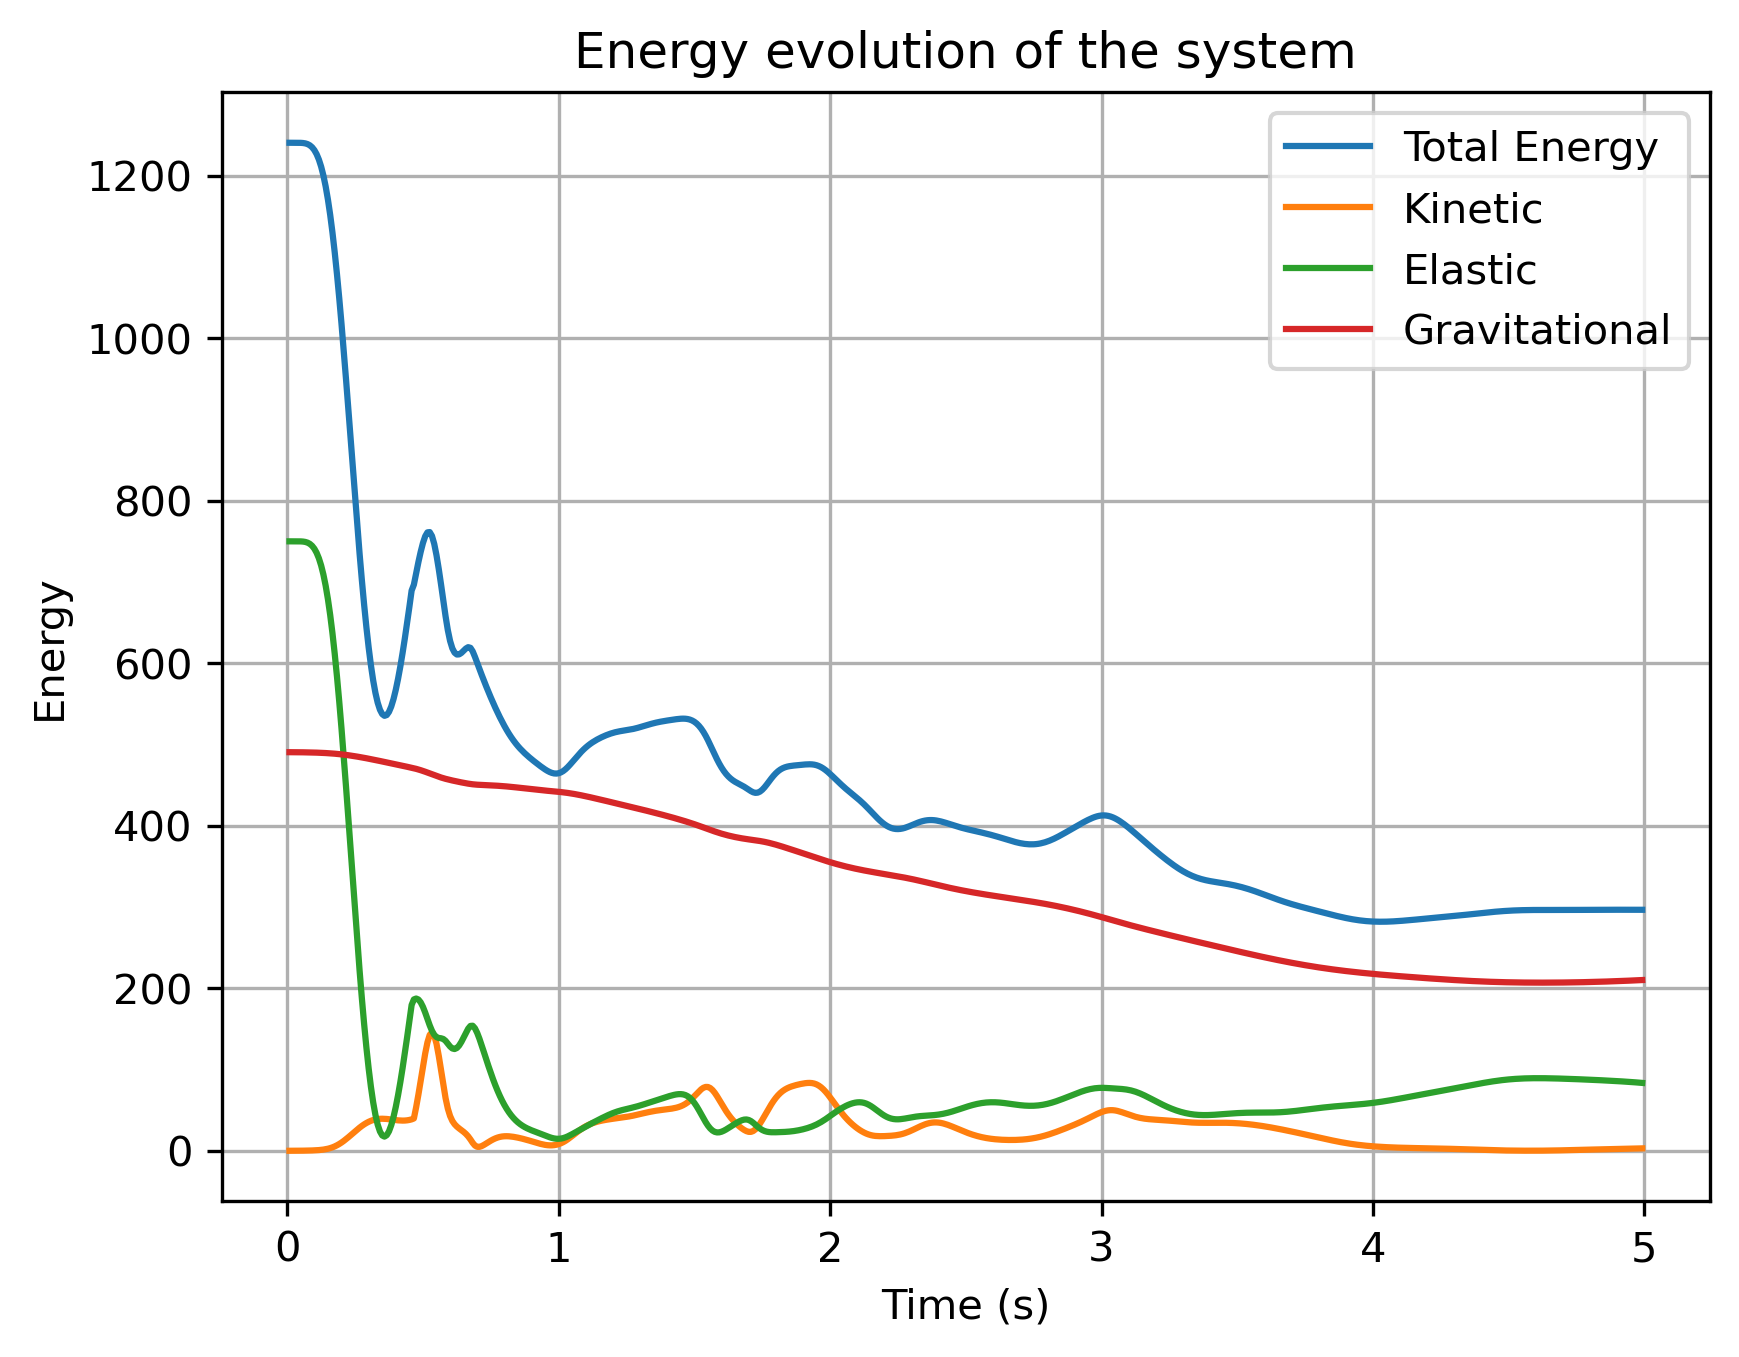
\includegraphics[width=\linewidth]{simulation_data_len1_k100_energy_5s}
\caption{Energy evolution for spring stiffness $k=100$ with damping $c=k/20$ for the first 5 seconds. The plots show kinetic, elastic, gravitational, and total mechanical energy.}
\label{fig:energy_k100_5s}
\end{figure}

\begin{figure}[H]
\centering
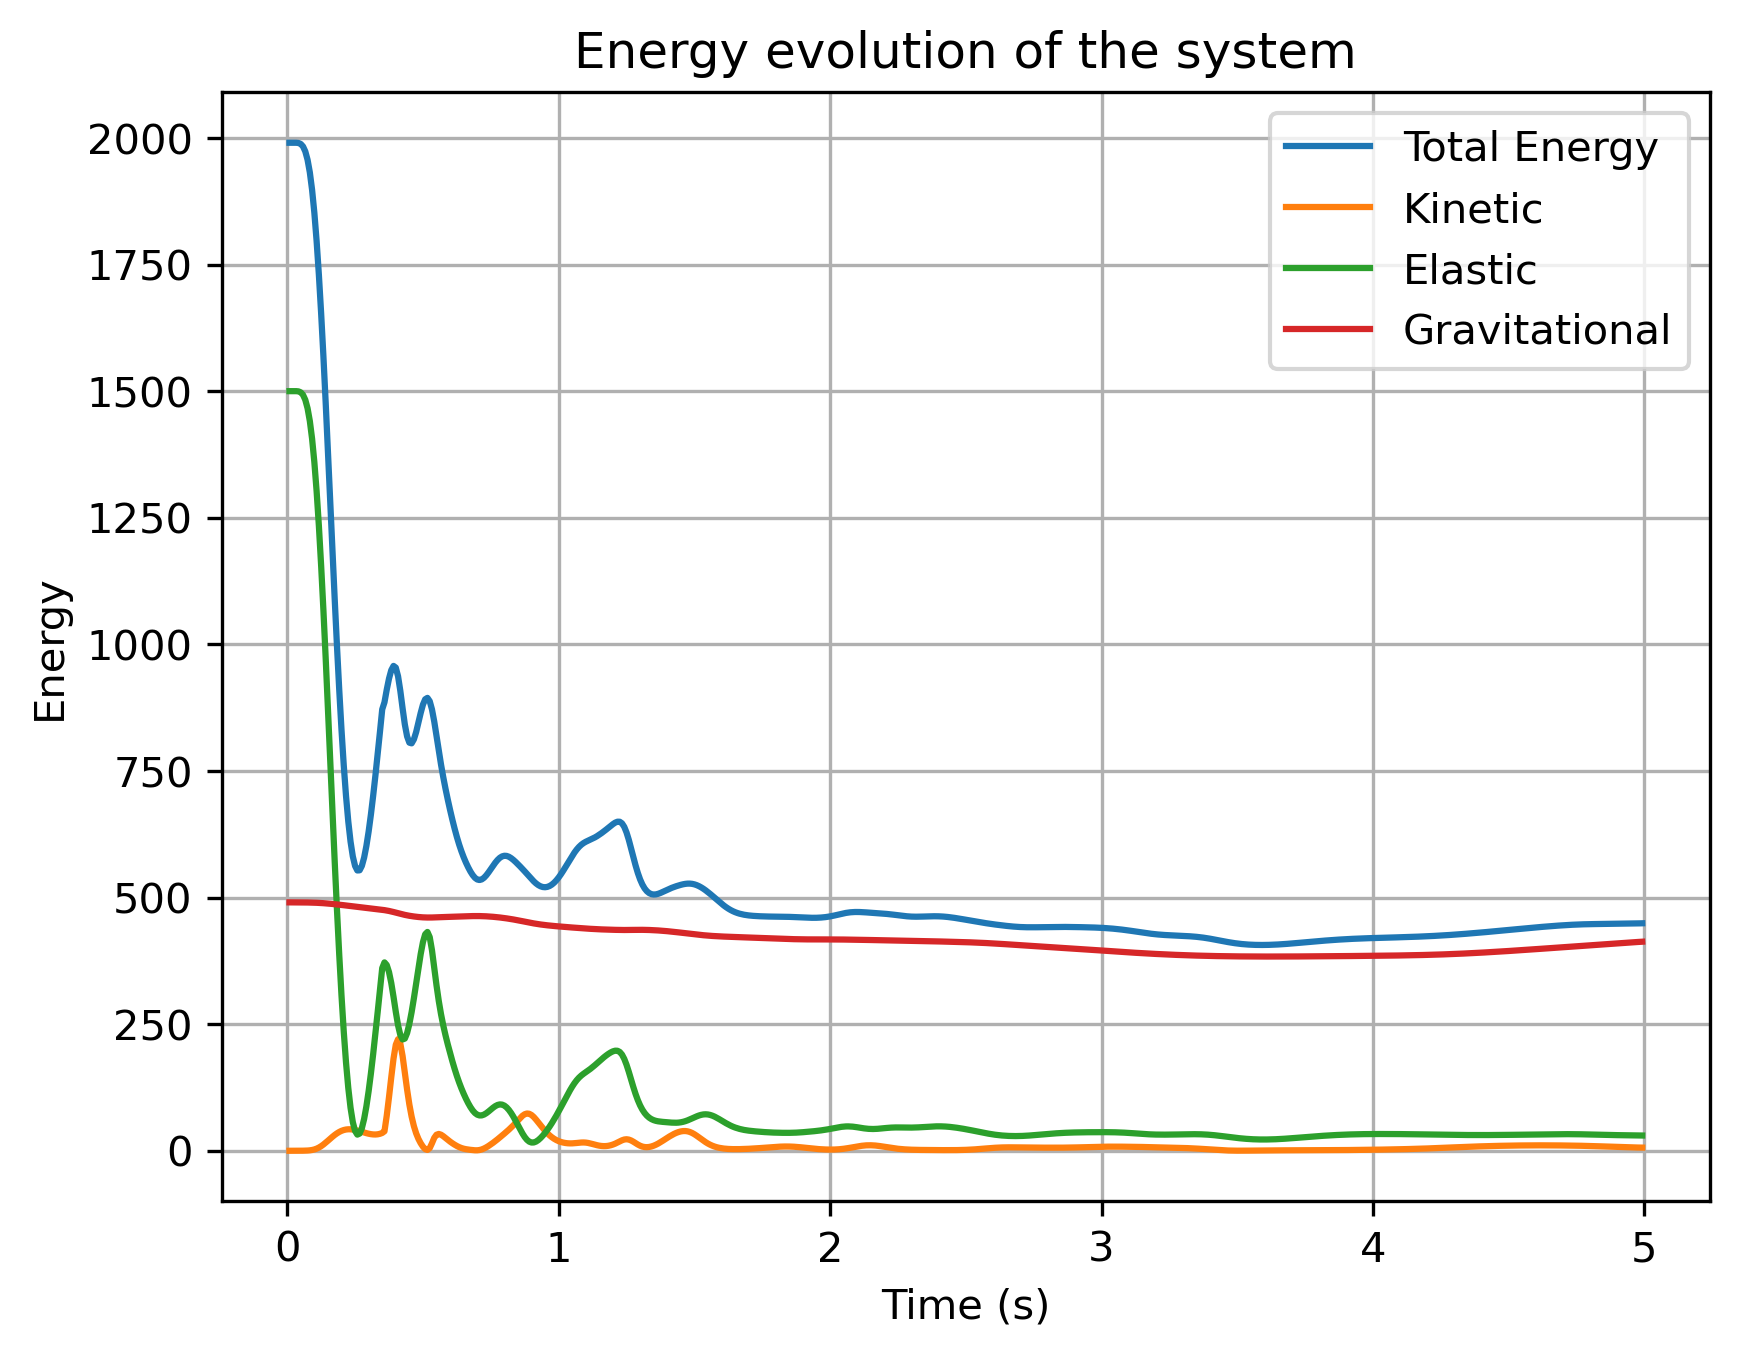
\includegraphics[width=\linewidth]{simulation_data_len1_k200_energy_5s}
\caption{Energy evolution for spring stiffness $k=200$ with damping $c=k/20$. Increased stiffness results in higher elastic energy storage.}
\label{fig:energy_k200_5s}
\end{figure}

\begin{figure}[H]
\centering
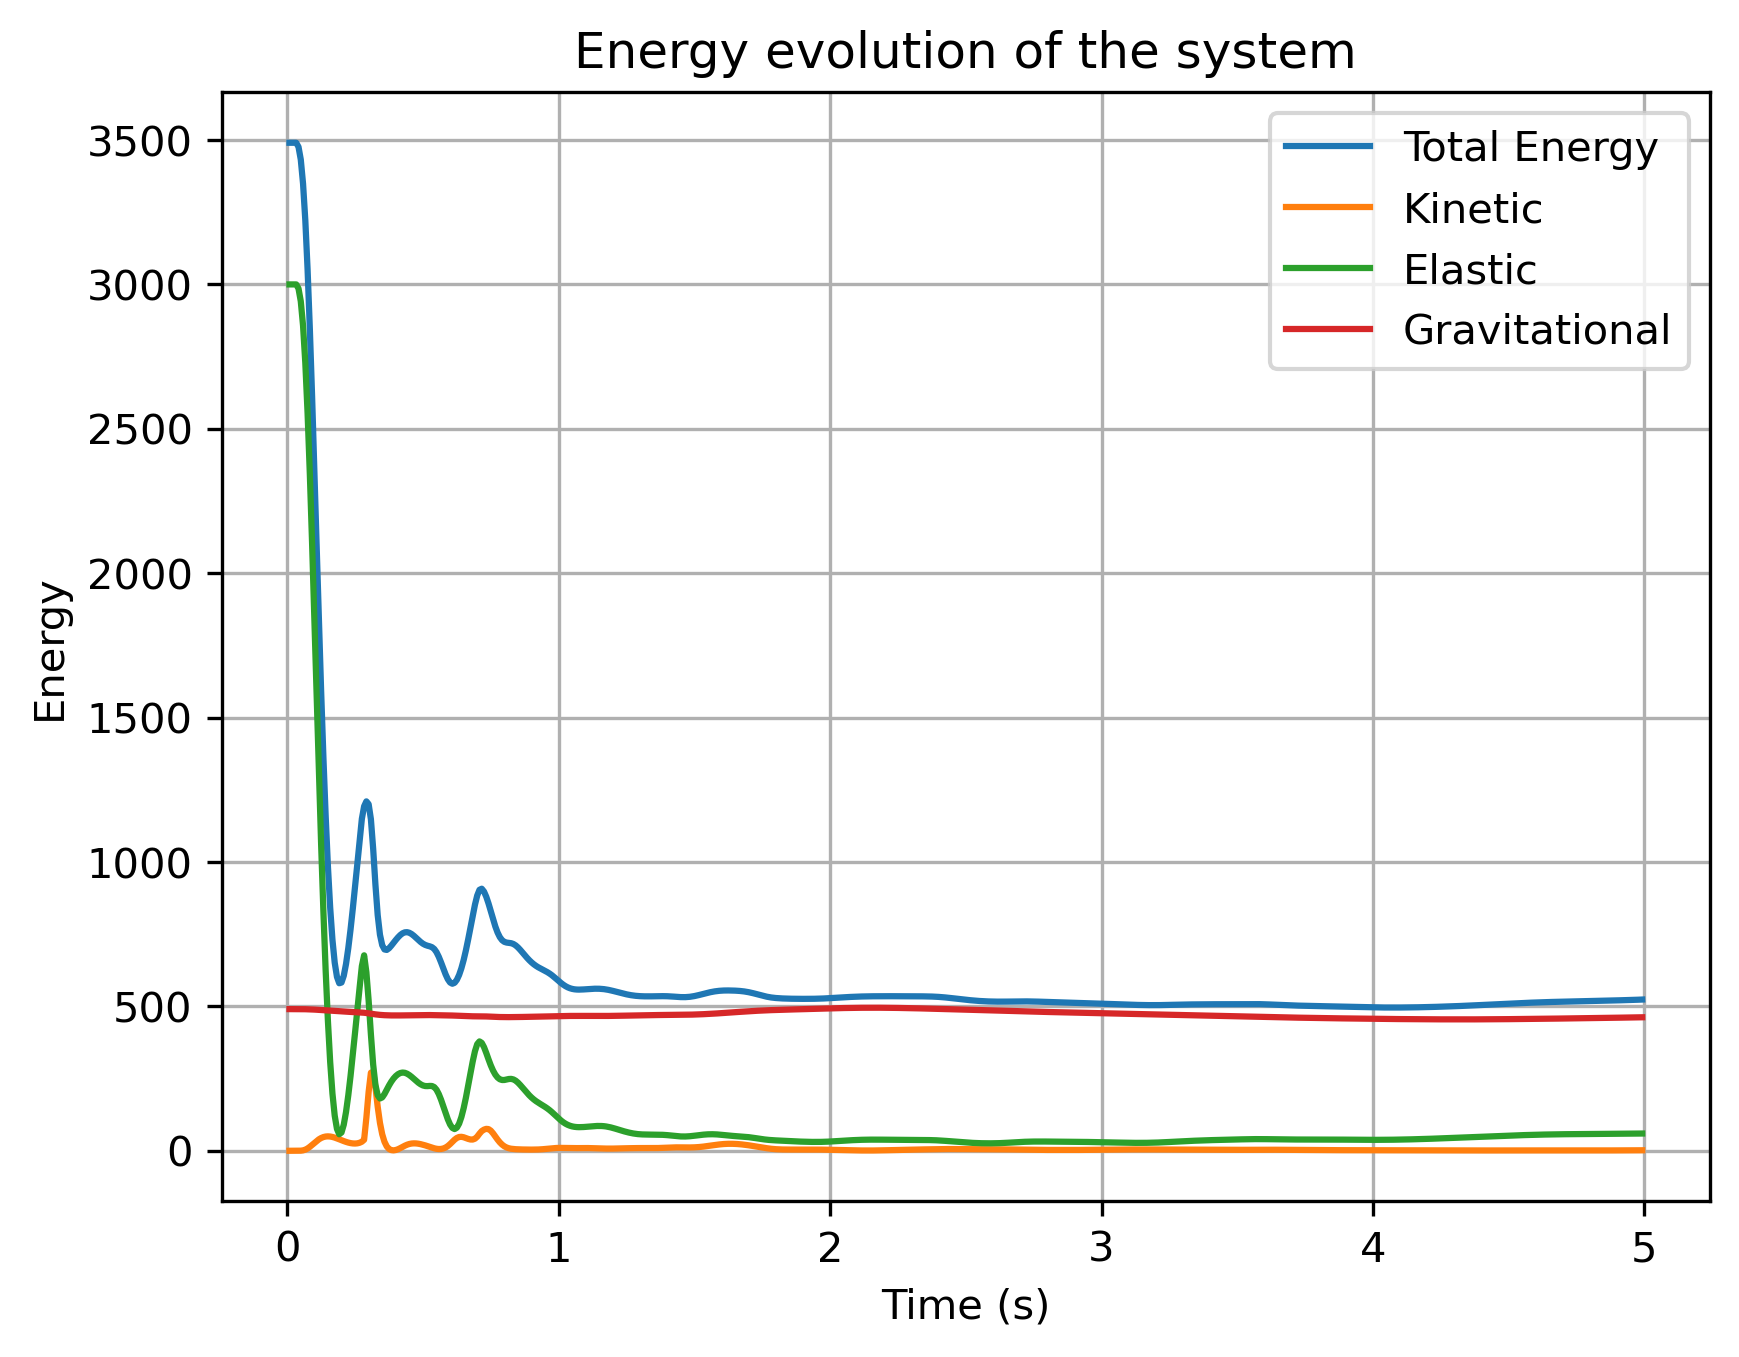
\includegraphics[width=\linewidth]{simulation_data_len1_k400_energy_5s}
\caption{Energy evolution for spring stiffness $k=400$ with damping $c=k/20$. The stiffer system exhibits more rapid energy exchange.}
\label{fig:energy_k400_5s}
\end{figure}

Figures~\ref{fig:energy_k100_5s}--\ref{fig:energy_k400_5s} show the energy evolution during the first $5$ seconds of simulation. In all cases, the system begins with a large elastic potential energy due to the compressed springs. This energy is rapidly released as the system accelerates toward equilibrium, producing a sharp increase in kinetic energy.

Simultaneously, gravitational potential energy decreases as the particles fall under gravity. The early-time behavior is dominated by this rapid redistribution of energy, resulting in pronounced oscillations as elastic and kinetic energies exchange. These oscillations are characteristic of underdamped second-order systems and are consistent with both the Newtonian force-based formulation and the Lagrangian energy-based formulation derived earlier. The exchange also exhibits a chaotic motion due to the influence of the neighboring particles on the recorded particle.

As expected, higher stiffness values result in larger initial elastic energies and higher-frequency oscillations. Despite the differing magnitudes, the qualitative behavior remains consistent across all stiffness values.

\subsection{Short-Term Position Response}
\label{Sec7.3:ShortTermPosition}

\begin{figure}[H]
\centering
\begin{subfigure}[b]{0.48\linewidth}
    \centering
    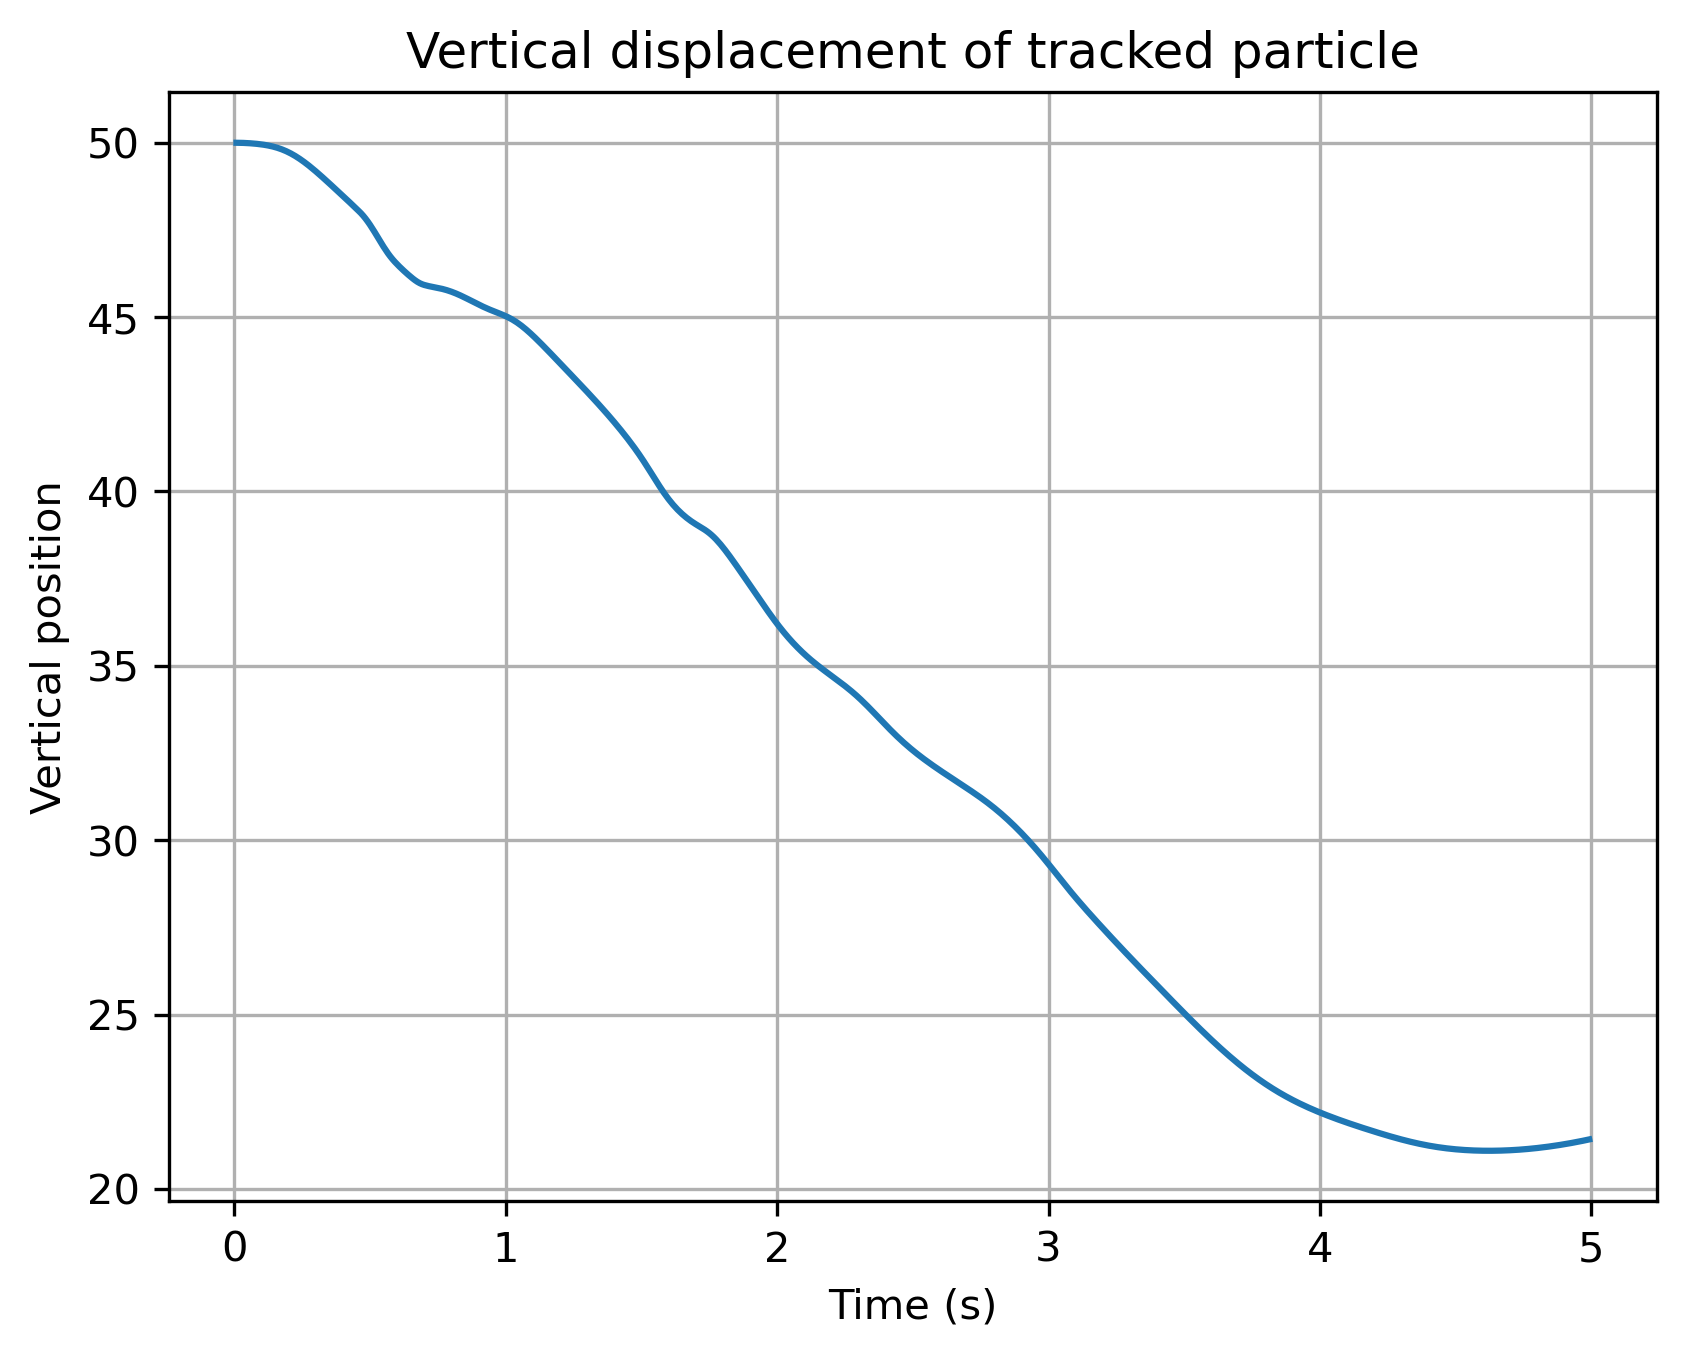
\includegraphics[width=\linewidth]{simulation_data_len1_k100_pos_5s}
    \caption{First 5 seconds}
\end{subfigure}
\hfill
\begin{subfigure}[b]{0.48\linewidth}
    \centering
    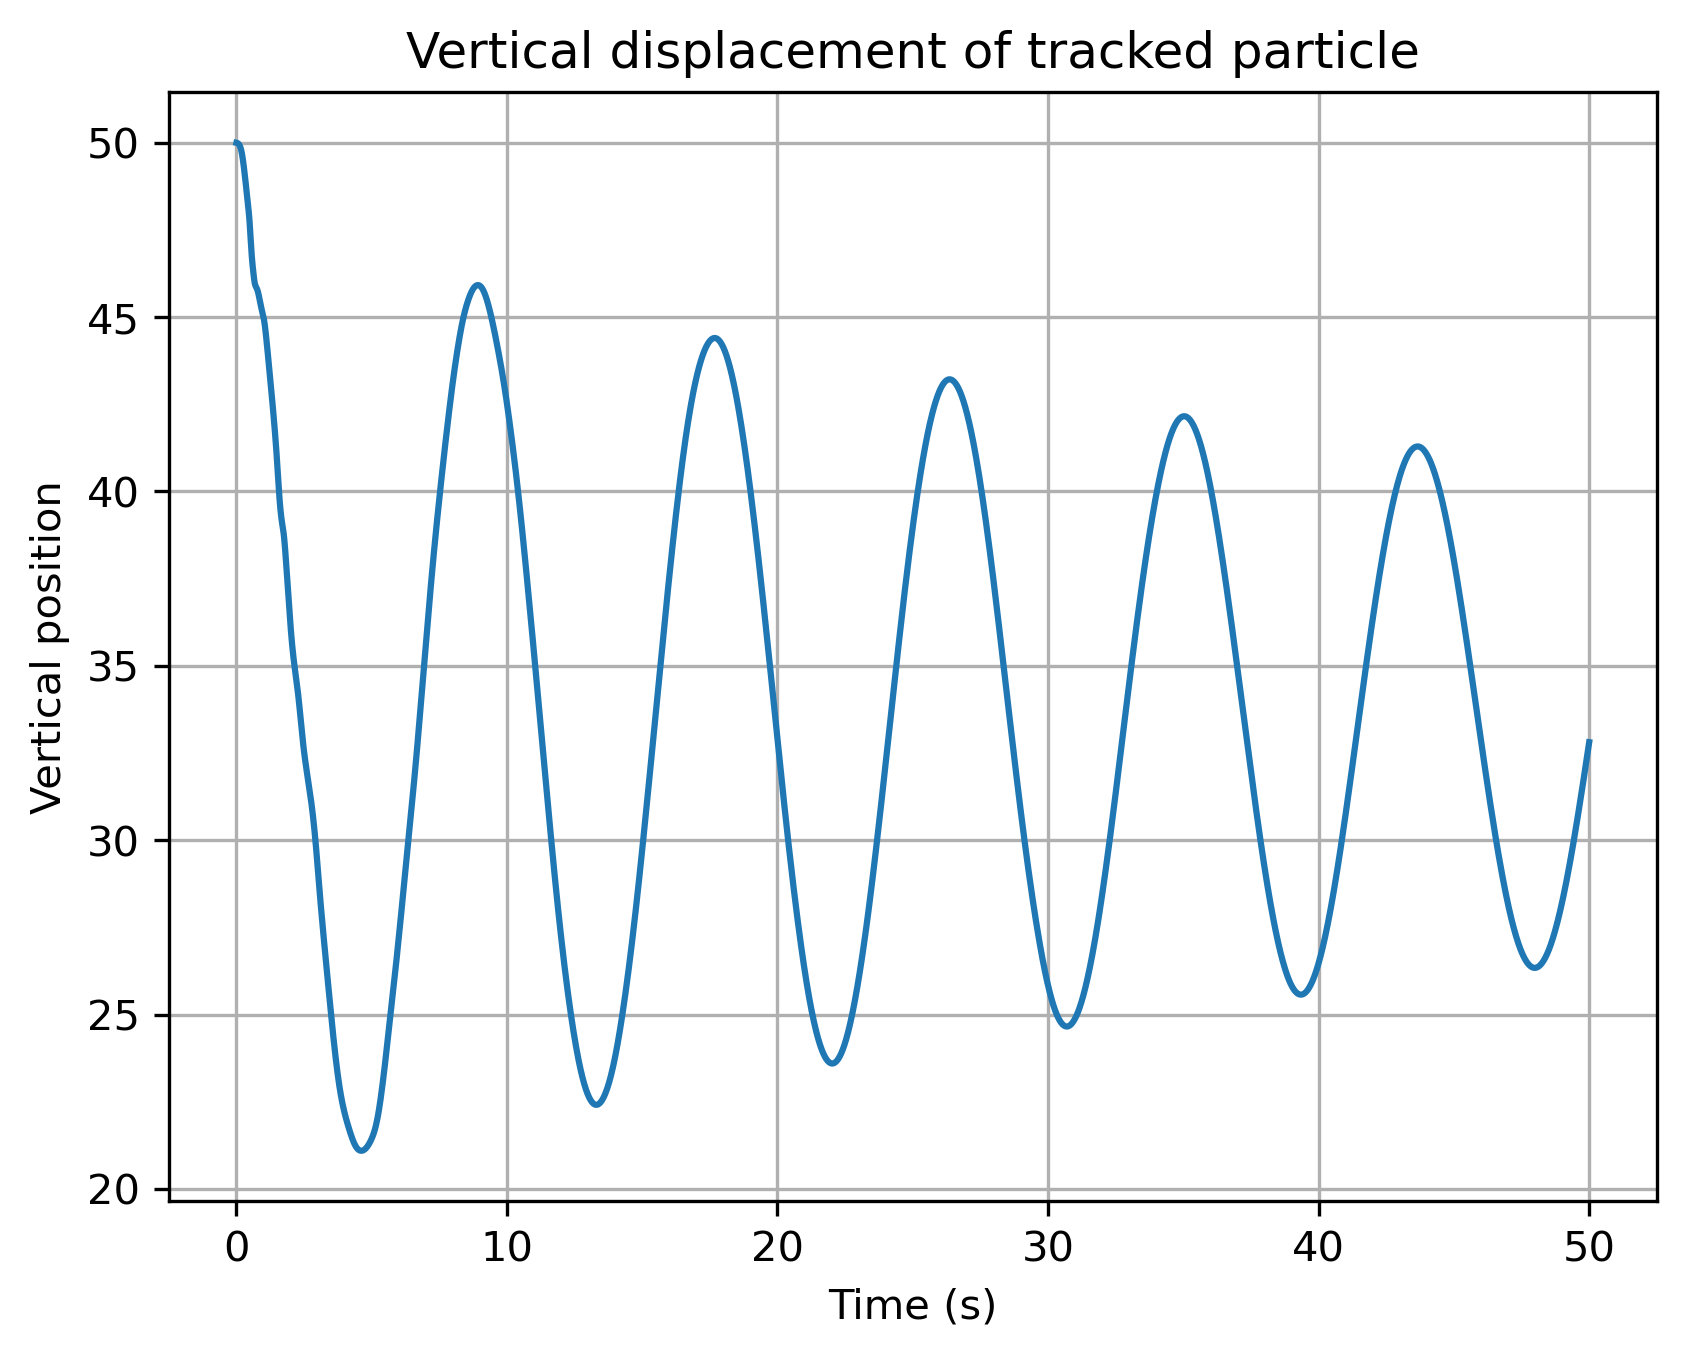
\includegraphics[width=\linewidth]{simulation_data_len1_k100_pos_50s}
    \caption{First 50 seconds}
\end{subfigure}
\caption{Position displacement for spring stiffness $k=100$ with damping $c=k/20$.}
\label{fig:pos_k100_s}
\end{figure}

\begin{figure}[H]
\centering
\begin{subfigure}[b]{0.48\linewidth}
    \centering
    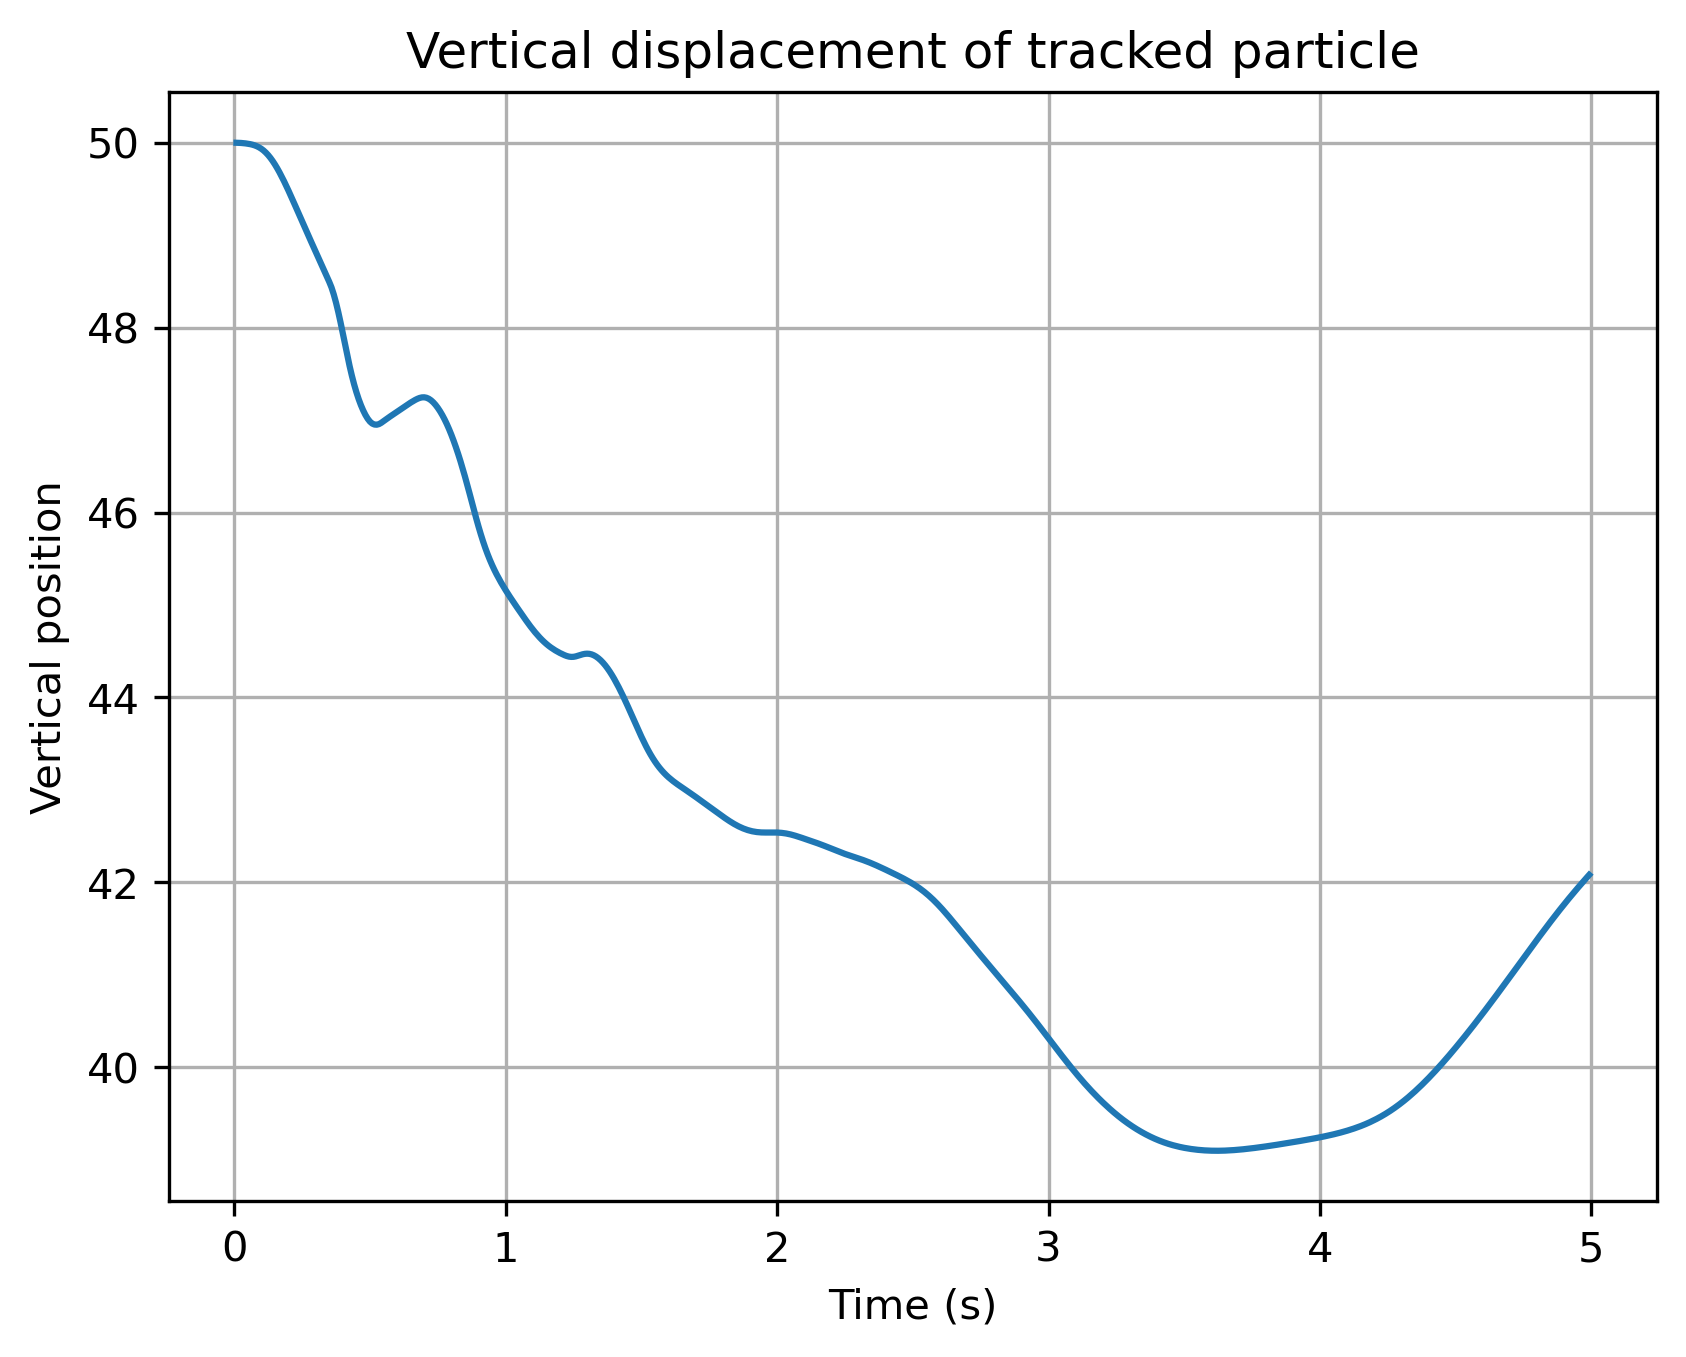
\includegraphics[width=\linewidth]{simulation_data_len1_k200_pos_5s.png}
    \caption{First 5 seconds}
\end{subfigure}
\hfill
\begin{subfigure}[b]{0.48\linewidth}
    \centering
    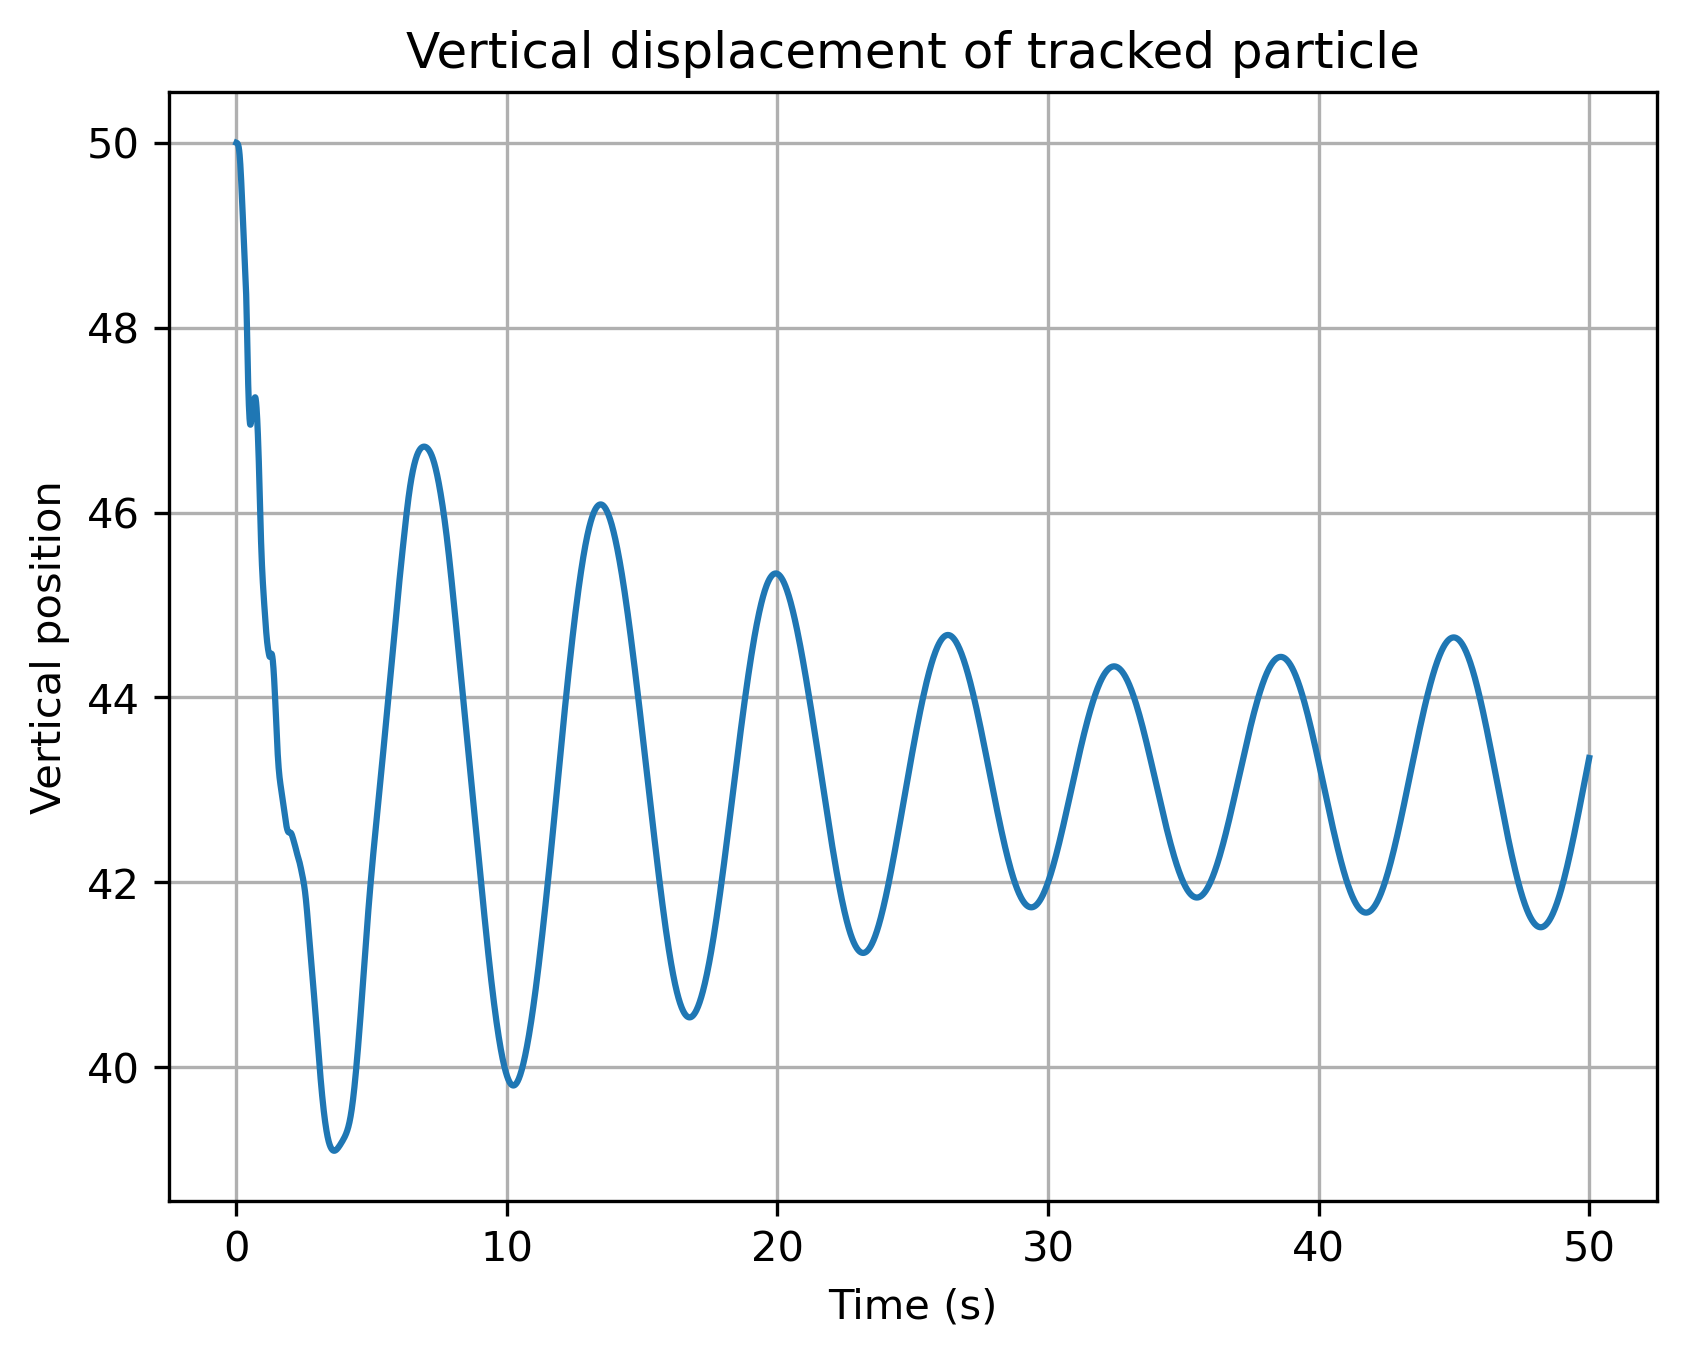
\includegraphics[width=\linewidth]{simulation_data_len1_k200_pos_50s.png}
    \caption{First 50 seconds}
\end{subfigure}
\caption{Position displacement for spring stiffness $k=200$ with damping $c=k/20$. Increased stiffness results in faster oscillations.}
\label{fig:pos_k200_s}
\end{figure}

\begin{figure}[H]
\centering
\begin{subfigure}[b]{0.48\linewidth}
    \centering
    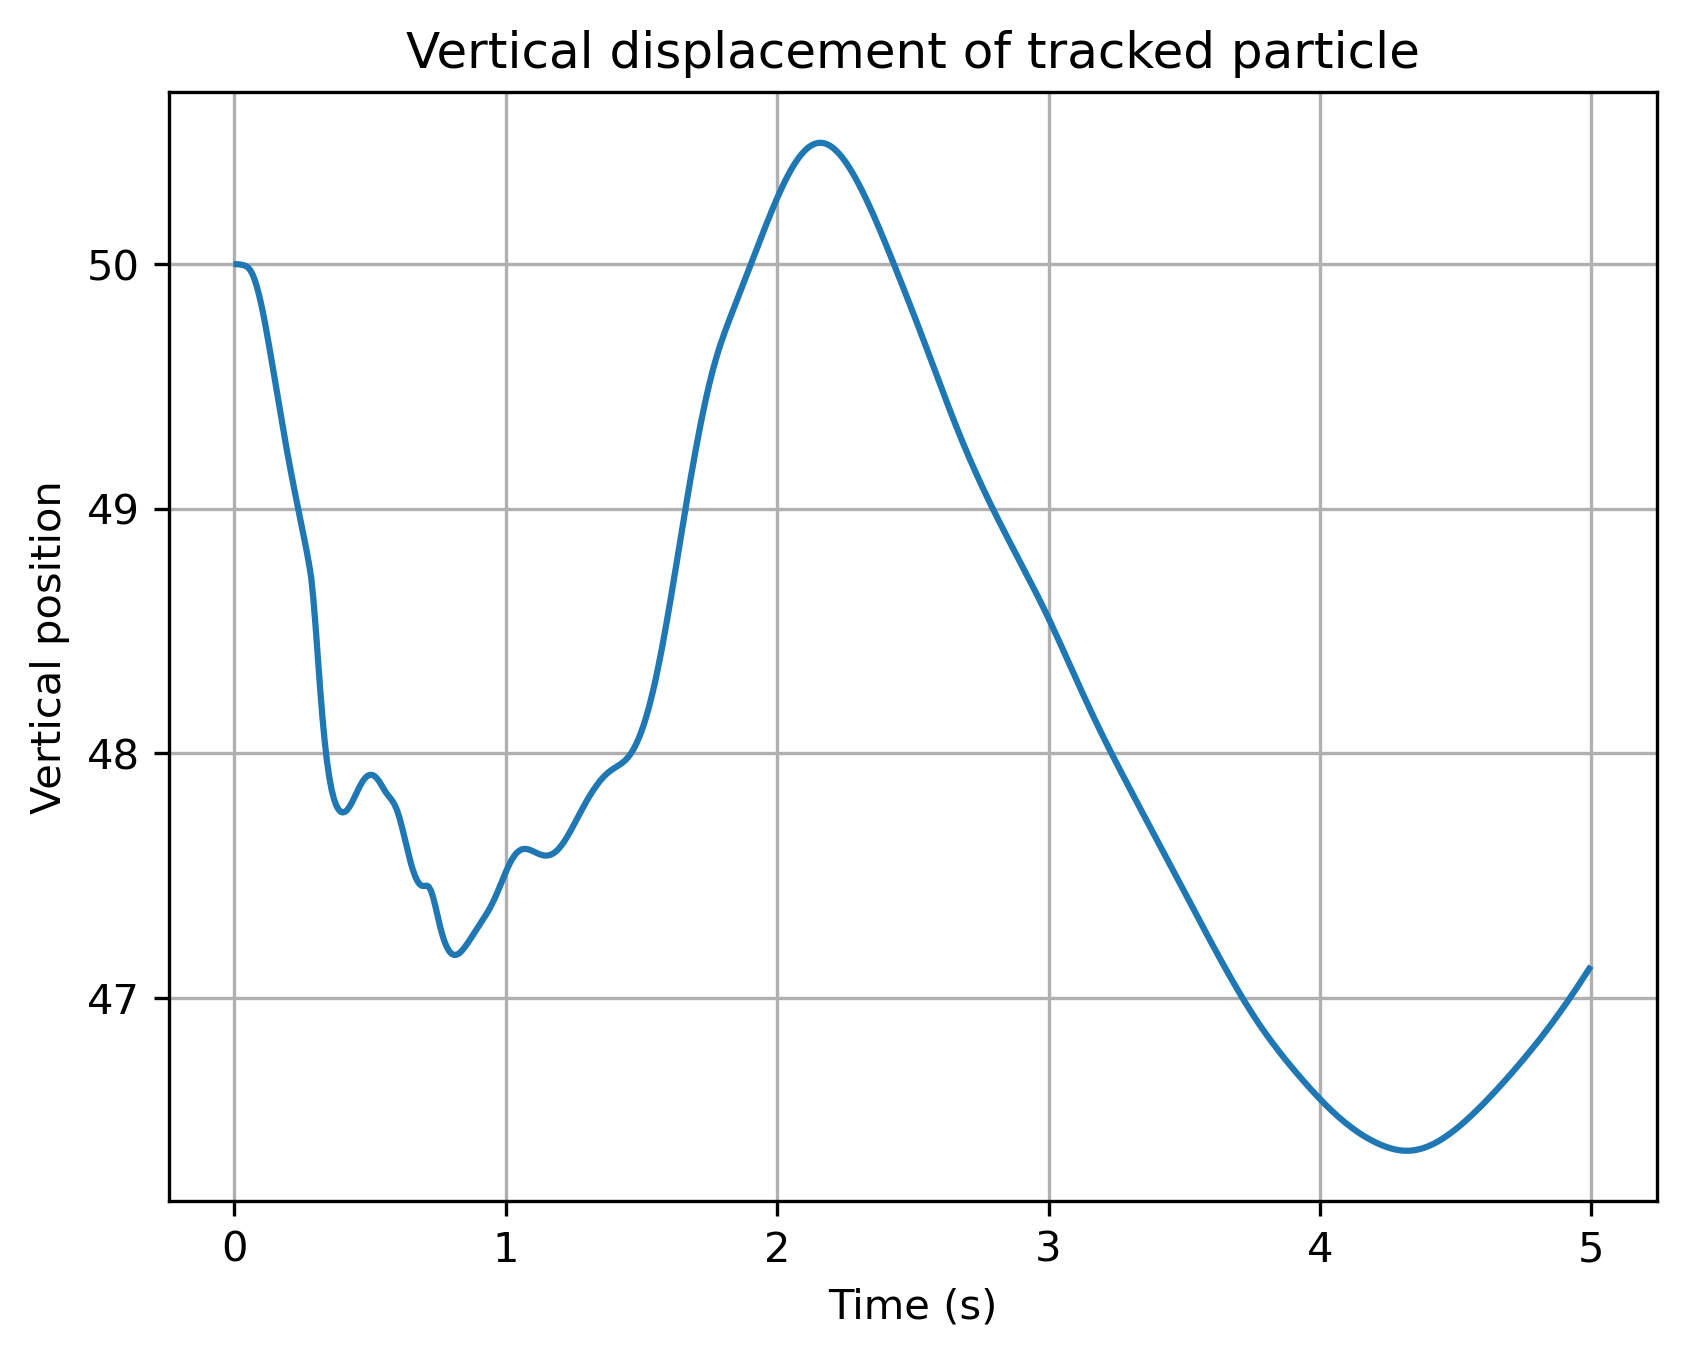
\includegraphics[width=\linewidth]{simulation_data_len1_k400_pos_5s}
    \caption{First 5 seconds}
\end{subfigure}
\hfill
\begin{subfigure}[b]{0.48\linewidth}
    \centering
    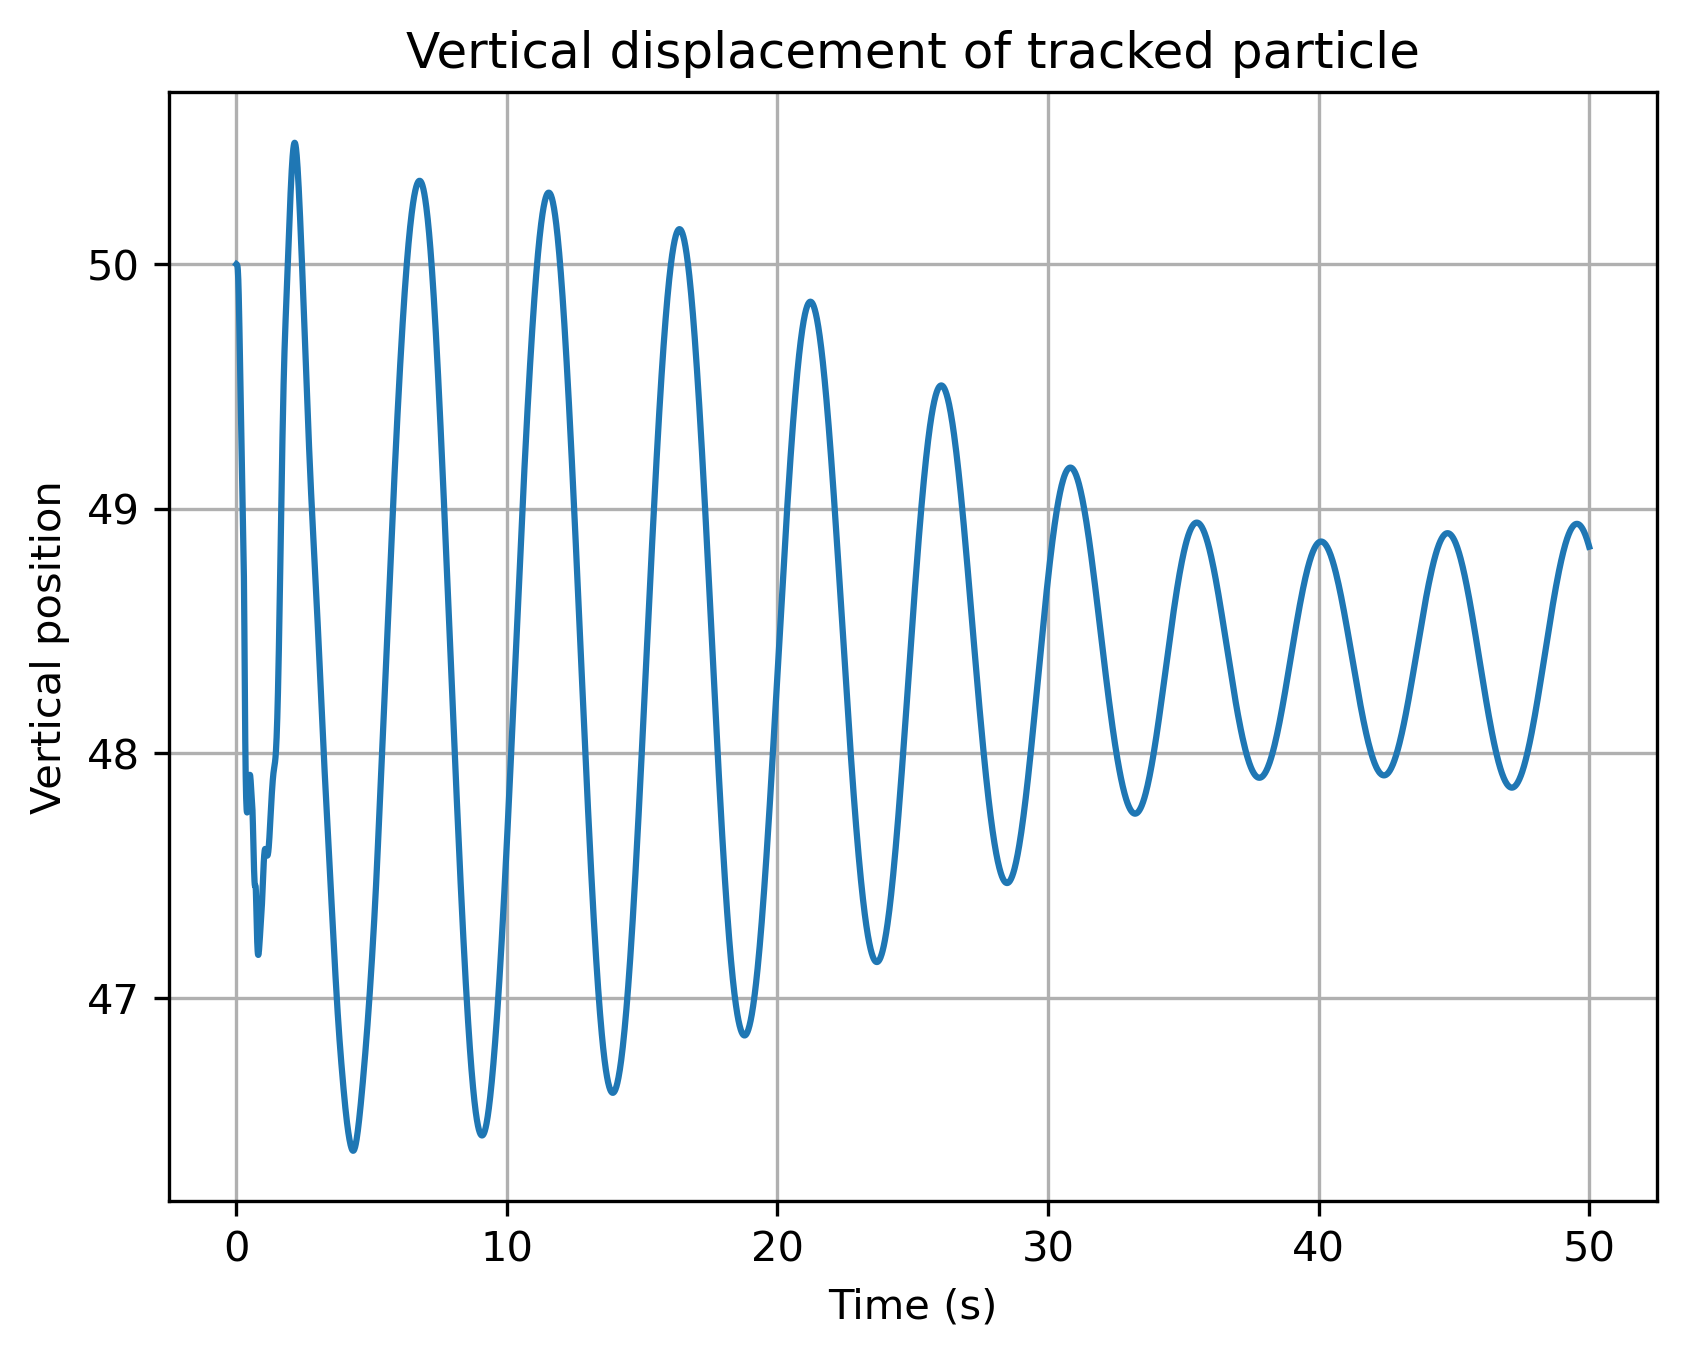
\includegraphics[width=\linewidth]{simulation_data_len1_k400_pos_50s}
    \caption{First 50 seconds}
\end{subfigure}
\caption{Position displacement for spring stiffness $k=400$ with damping $c=k/20$. The stiffer system exhibits very fast oscillations and stabilization towards equilibrium.}
\label{fig:pos_k400_s}
\end{figure}

Figures~\ref{fig:pos_k100_s}--\ref{fig:pos_k400_s} show the vertical displacement of a representative particle over the same $5$ second interval and extended $50$ second interval. The particle undergoes large-amplitude oscillations immediately after release, reflecting the strong restoring forces from the compressed springs.

The oscillation frequency increases with stiffness, while the amplitude decays over time due to viscous damping. This behavior aligns with the analytical expectation for a damped harmonic oscillator, with the effective stiffness governing the natural frequency and the damping term governing the decay rate.

\subsection{Long-Term Behavior and Dual Harmonic Oscillation}
\label{Sec7.4:LongTerm}

\begin{figure}[H]
\centering
\begin{subfigure}[b]{0.48\linewidth}
    \centering
    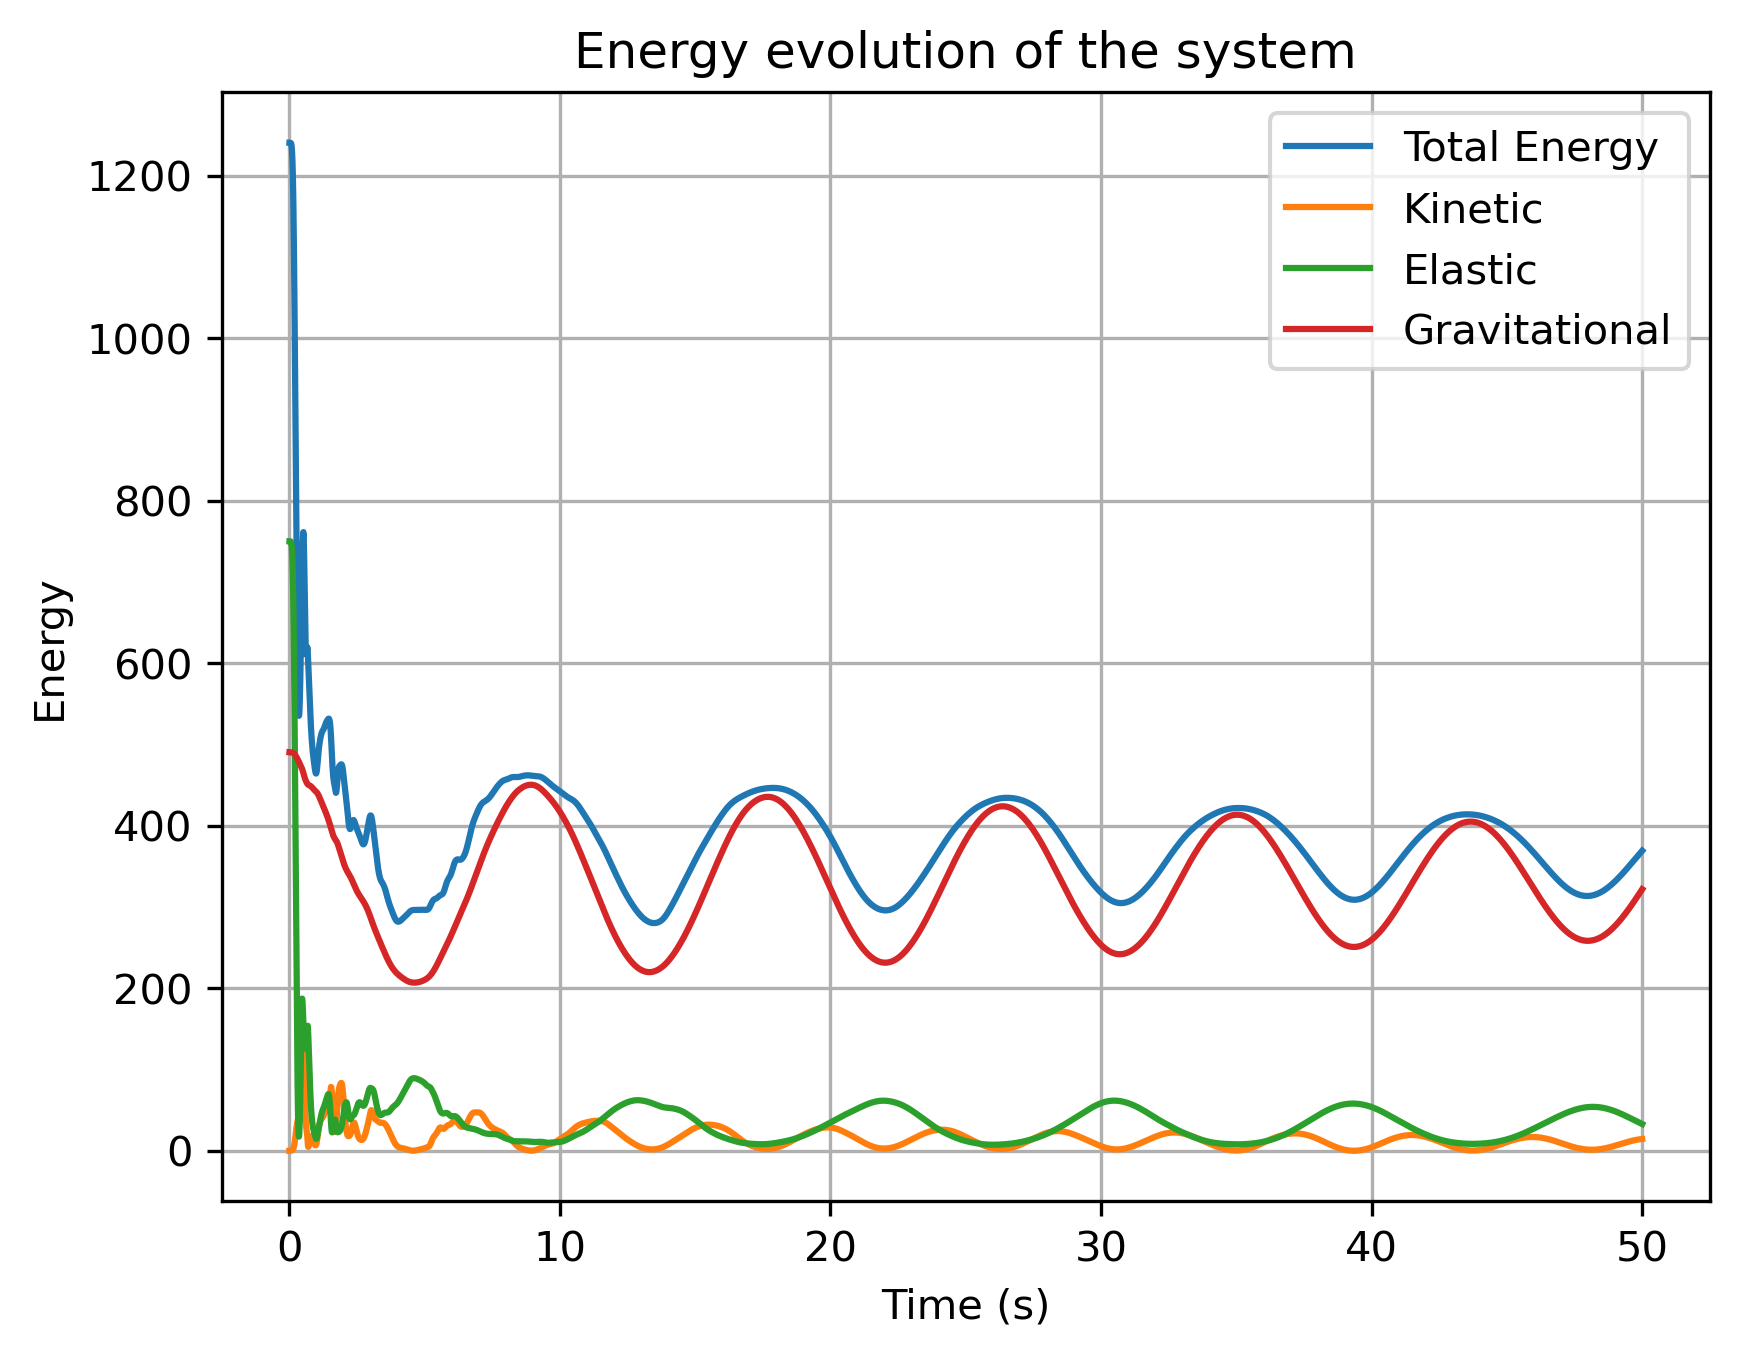
\includegraphics[width=\linewidth]{simulation_data_len1_k100_energy_50s}
    \caption{First 50 seconds (Repeat of \ref{fig:pos_k100_s}.b}
\end{subfigure}
\hfill
\begin{subfigure}[b]{0.48\linewidth}
    \centering
    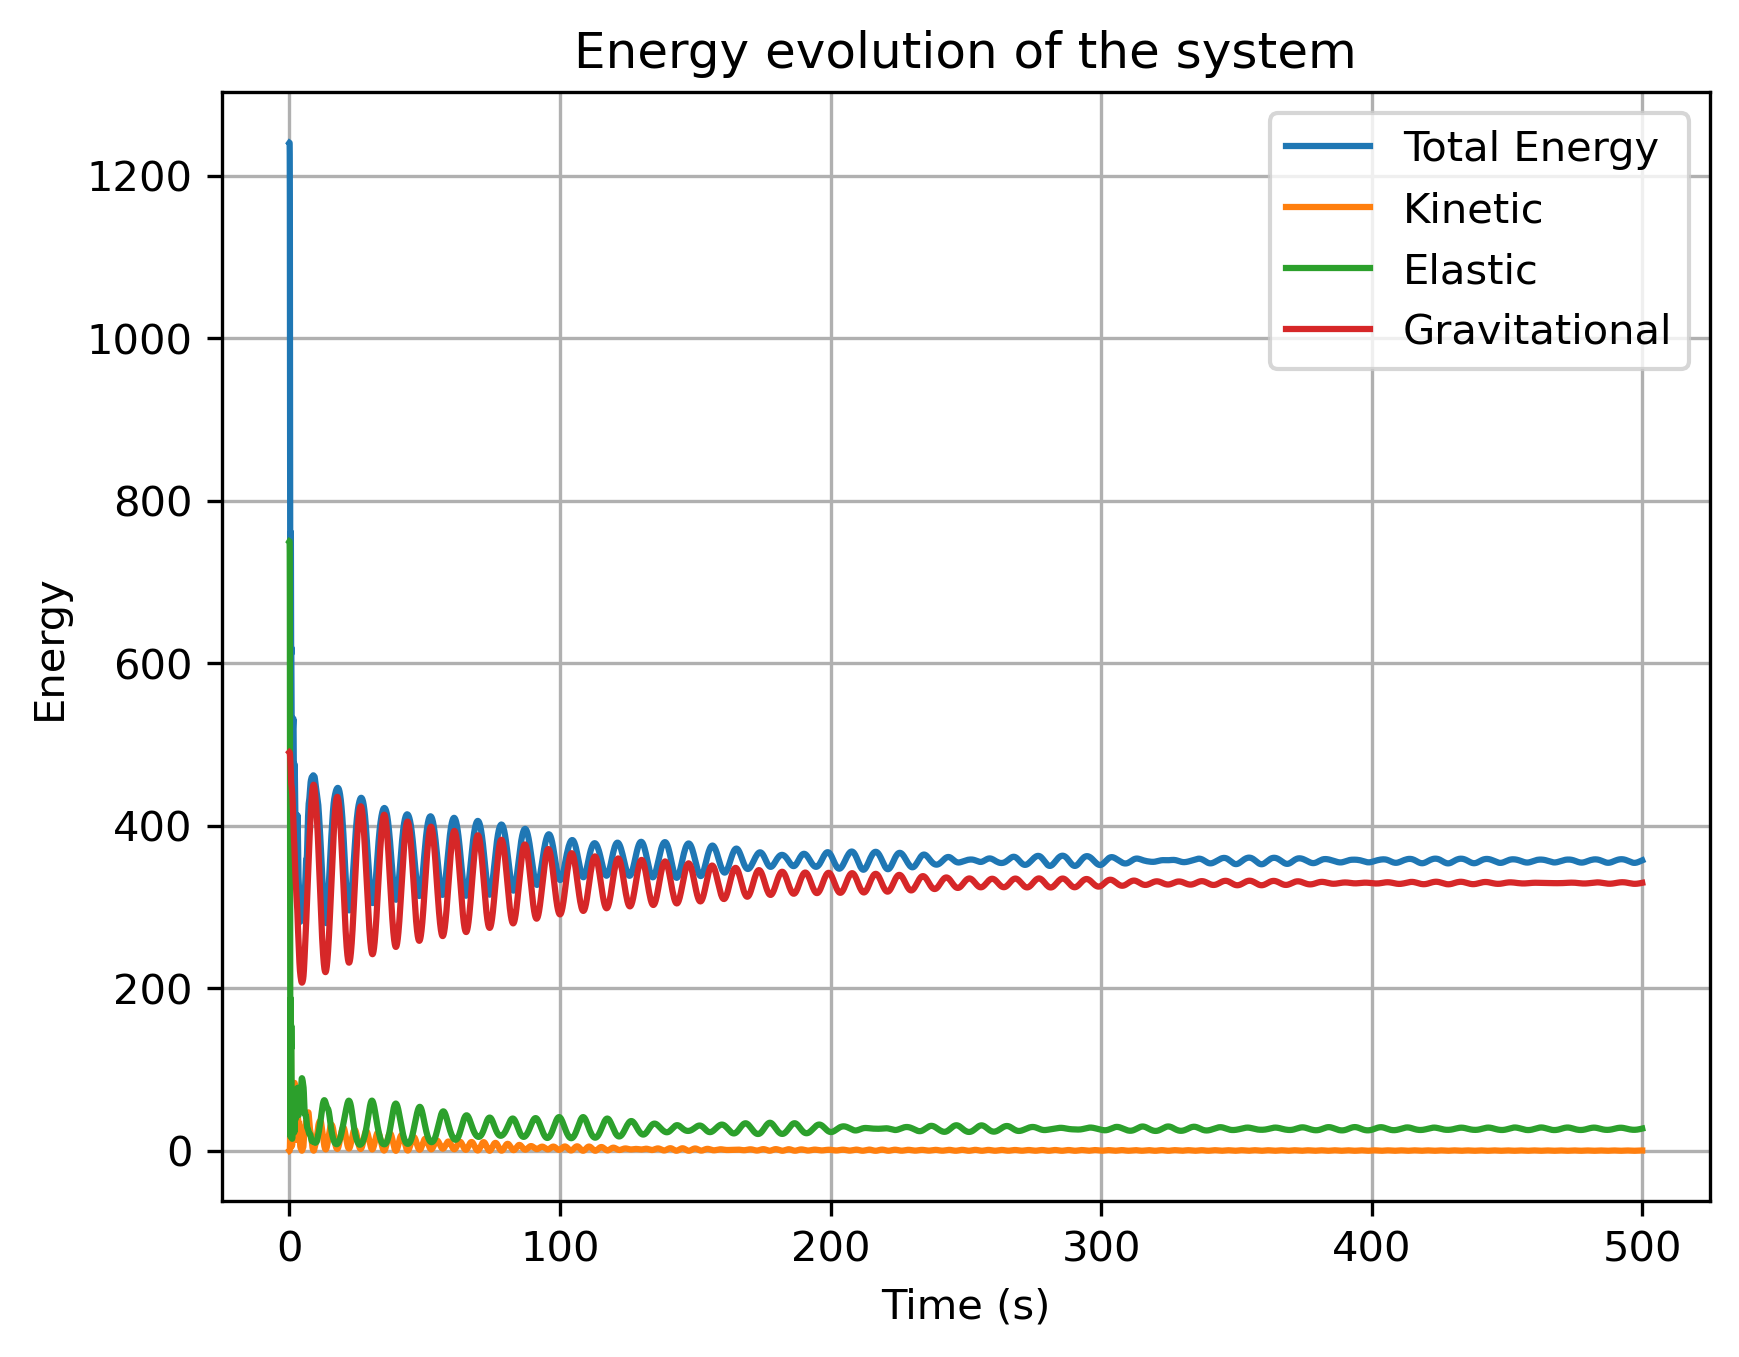
\includegraphics[width=\linewidth]{simulation_data_len1_k100_energy_500s}
    \caption{First 500 seconds}
\end{subfigure}
\caption{Energy evolution for spring stiffness $k=100$ with damping $c=k/20$. The plots show kinetic, elastic, gravitational, and total mechanical energy.}
\label{fig:energy_k100_l}
\end{figure}

\begin{figure}[H]
\centering
\begin{subfigure}[b]{0.48\linewidth}
    \centering
    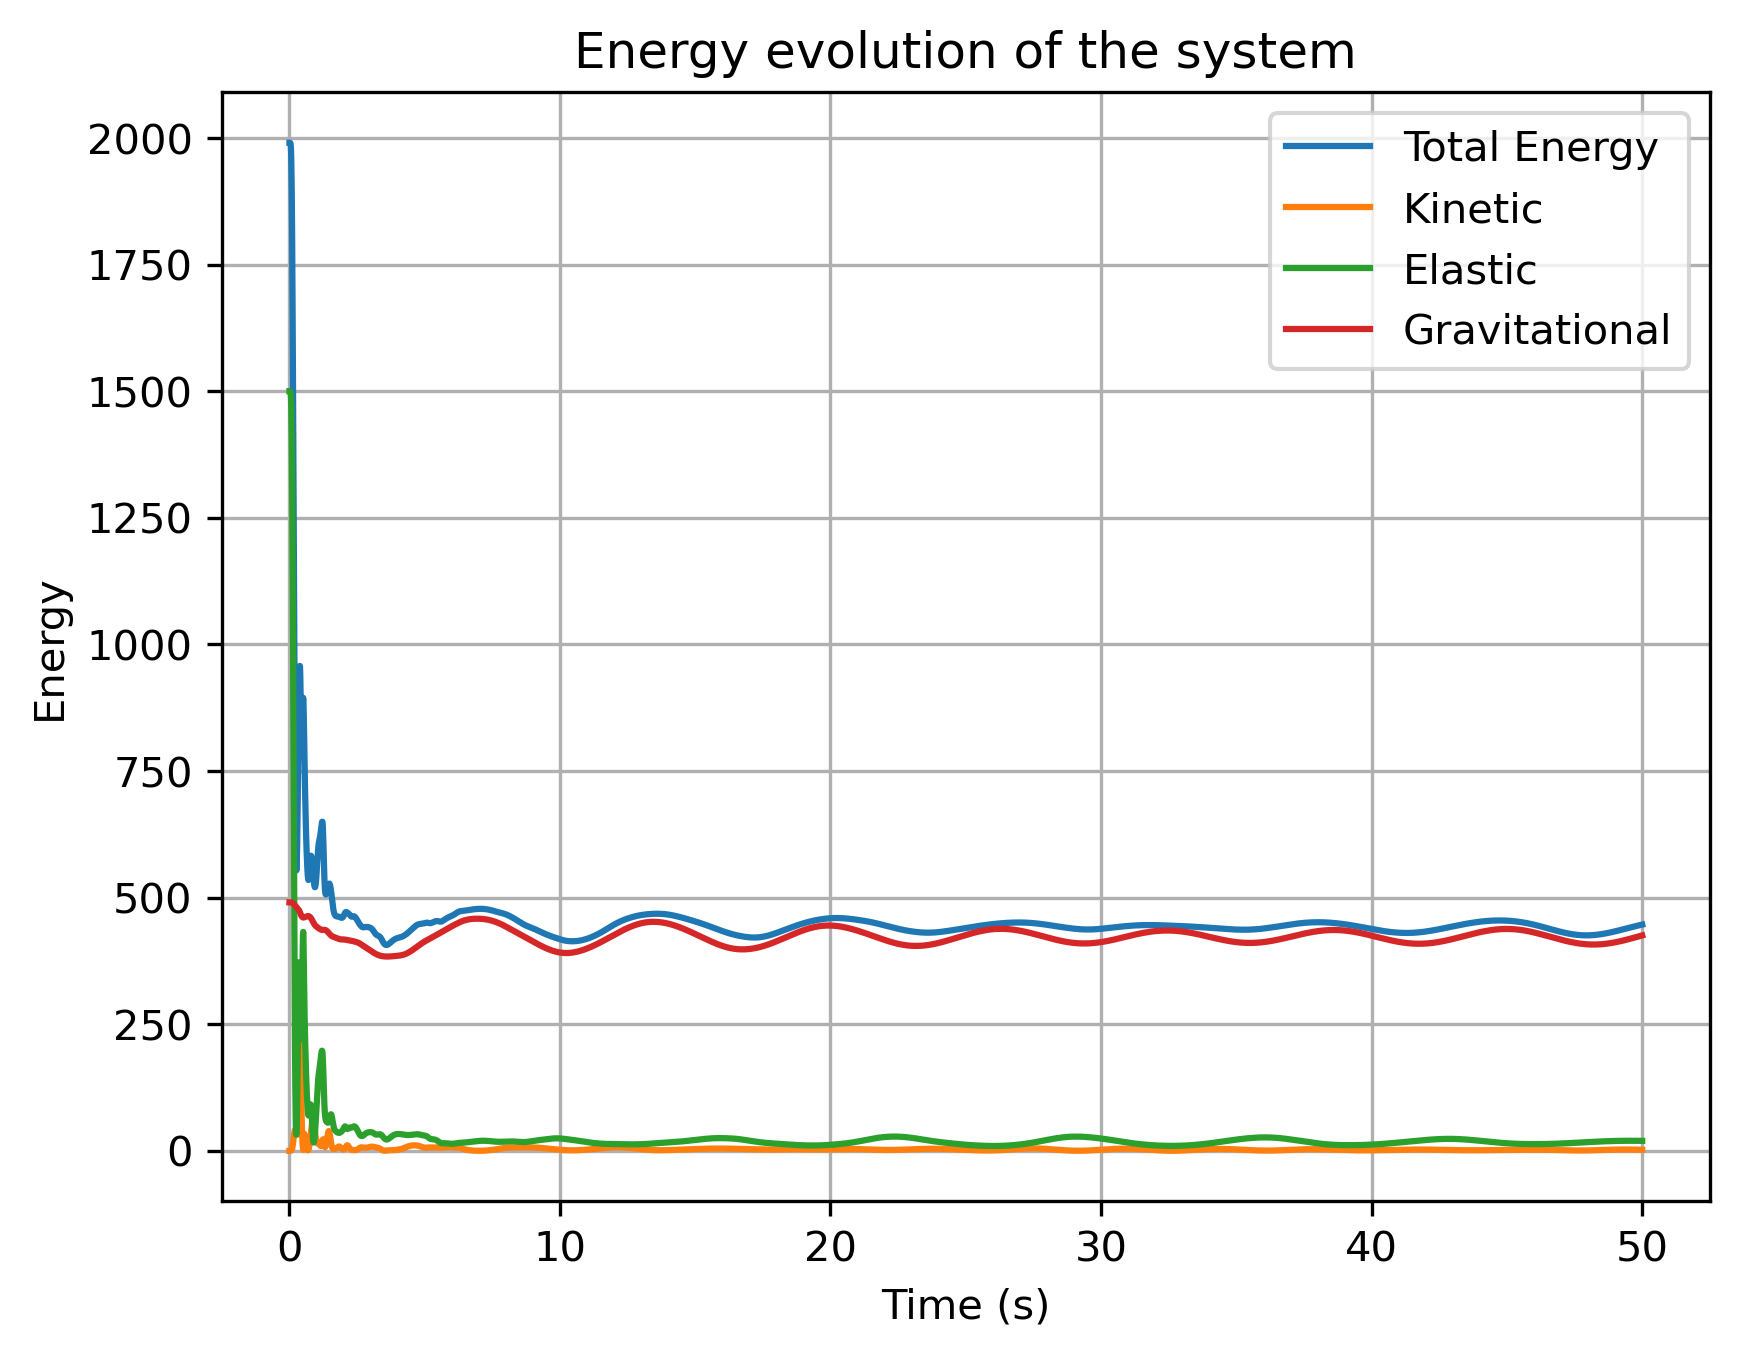
\includegraphics[width=\linewidth]{simulation_data_len1_k200_energy_50s}
    \caption{First 50 seconds (Repeat of \ref{fig:pos_k200_s}.b}
\end{subfigure}
\hfill
\begin{subfigure}[b]{0.48\linewidth}
    \centering
    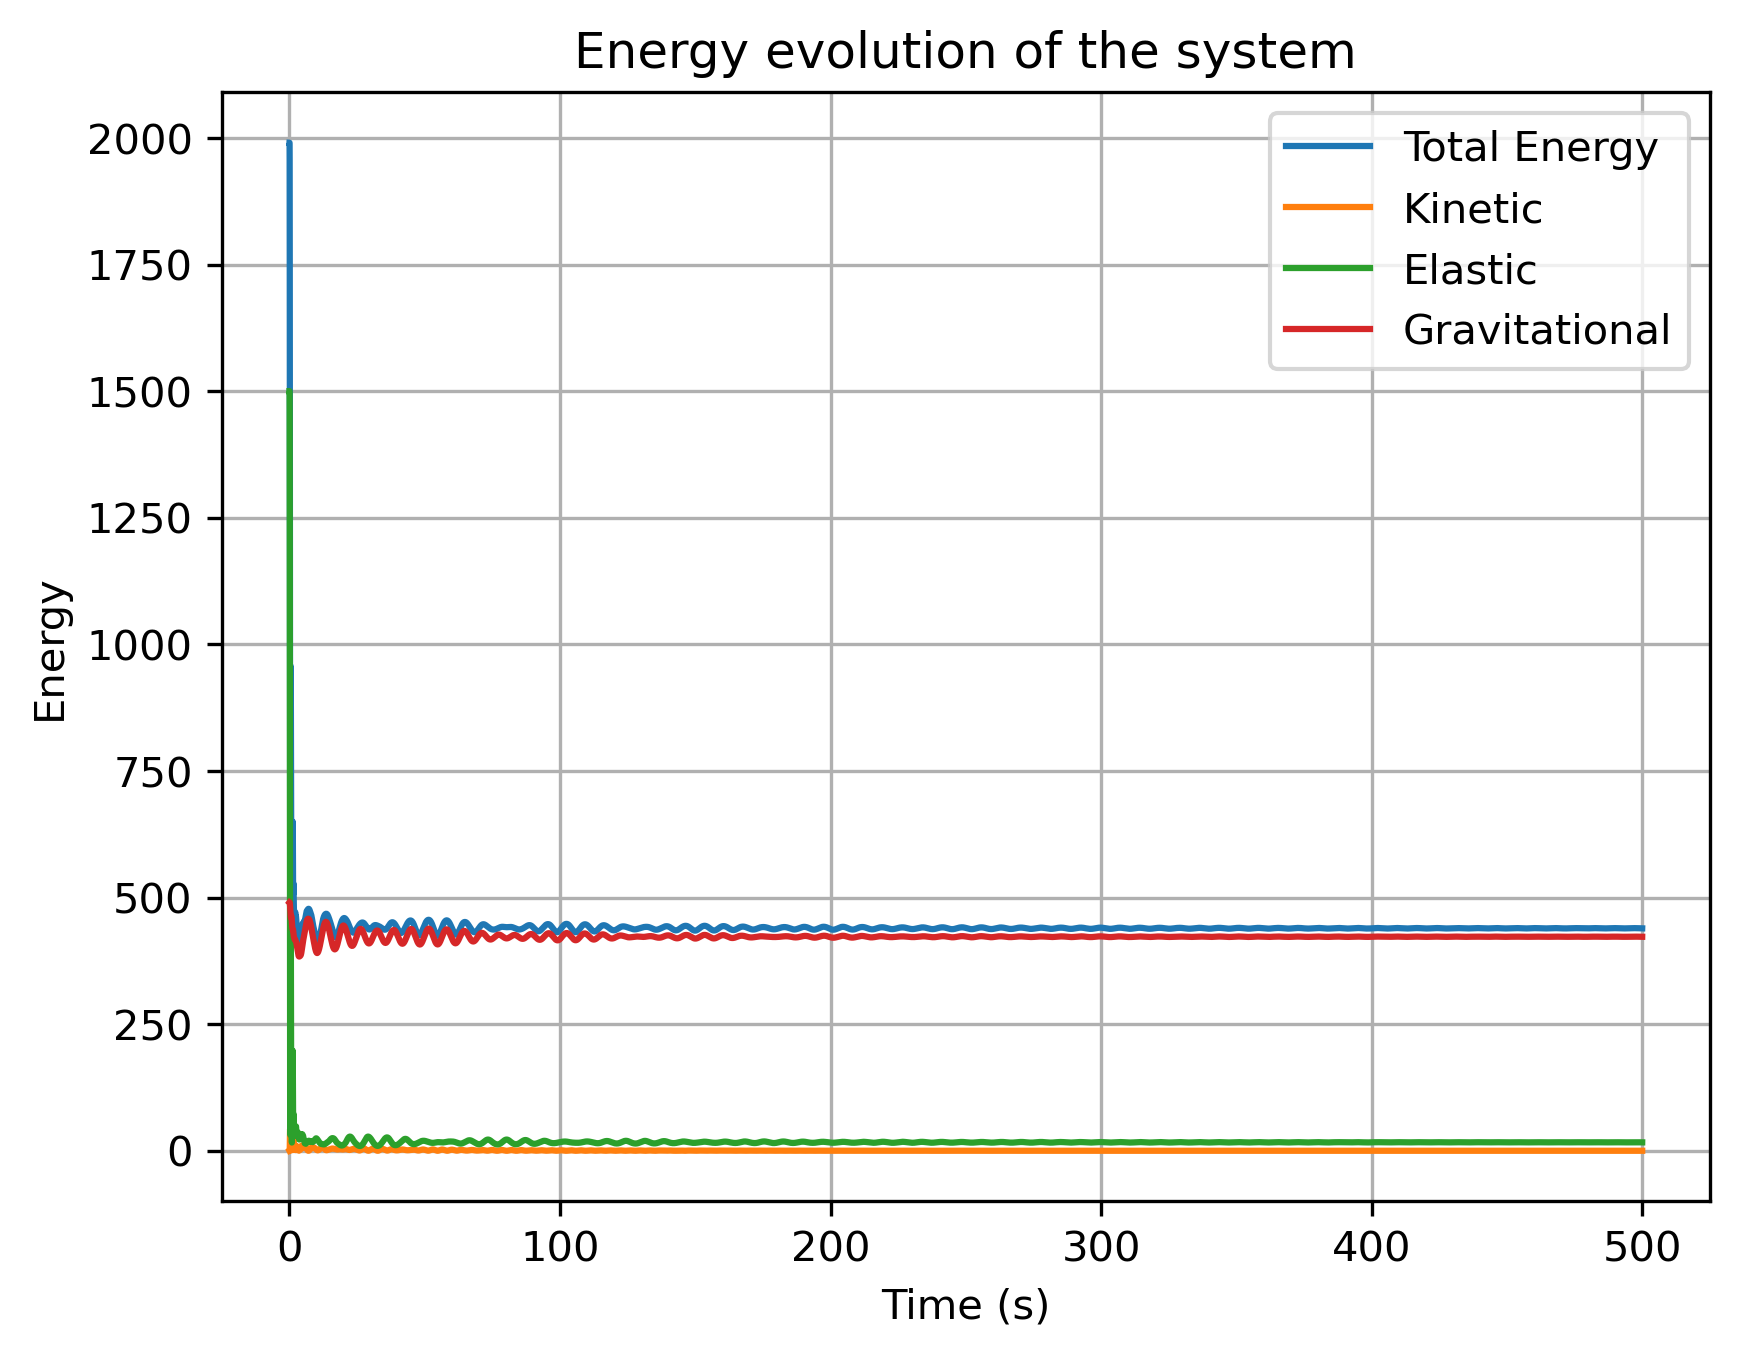
\includegraphics[width=\linewidth]{simulation_data_len1_k200_energy_500s}
    \caption{First 500 seconds}
\end{subfigure}
\caption{Energy evolution for spring stiffness $k=200$ with damping $c=k/20$. Increased stiffness results in faster oscillations and stabilization to equilibrium.}
\label{fig:energy_k200_l}
\end{figure}

\begin{figure}[H]
\centering
\begin{subfigure}[b]{0.48\linewidth}
    \centering
    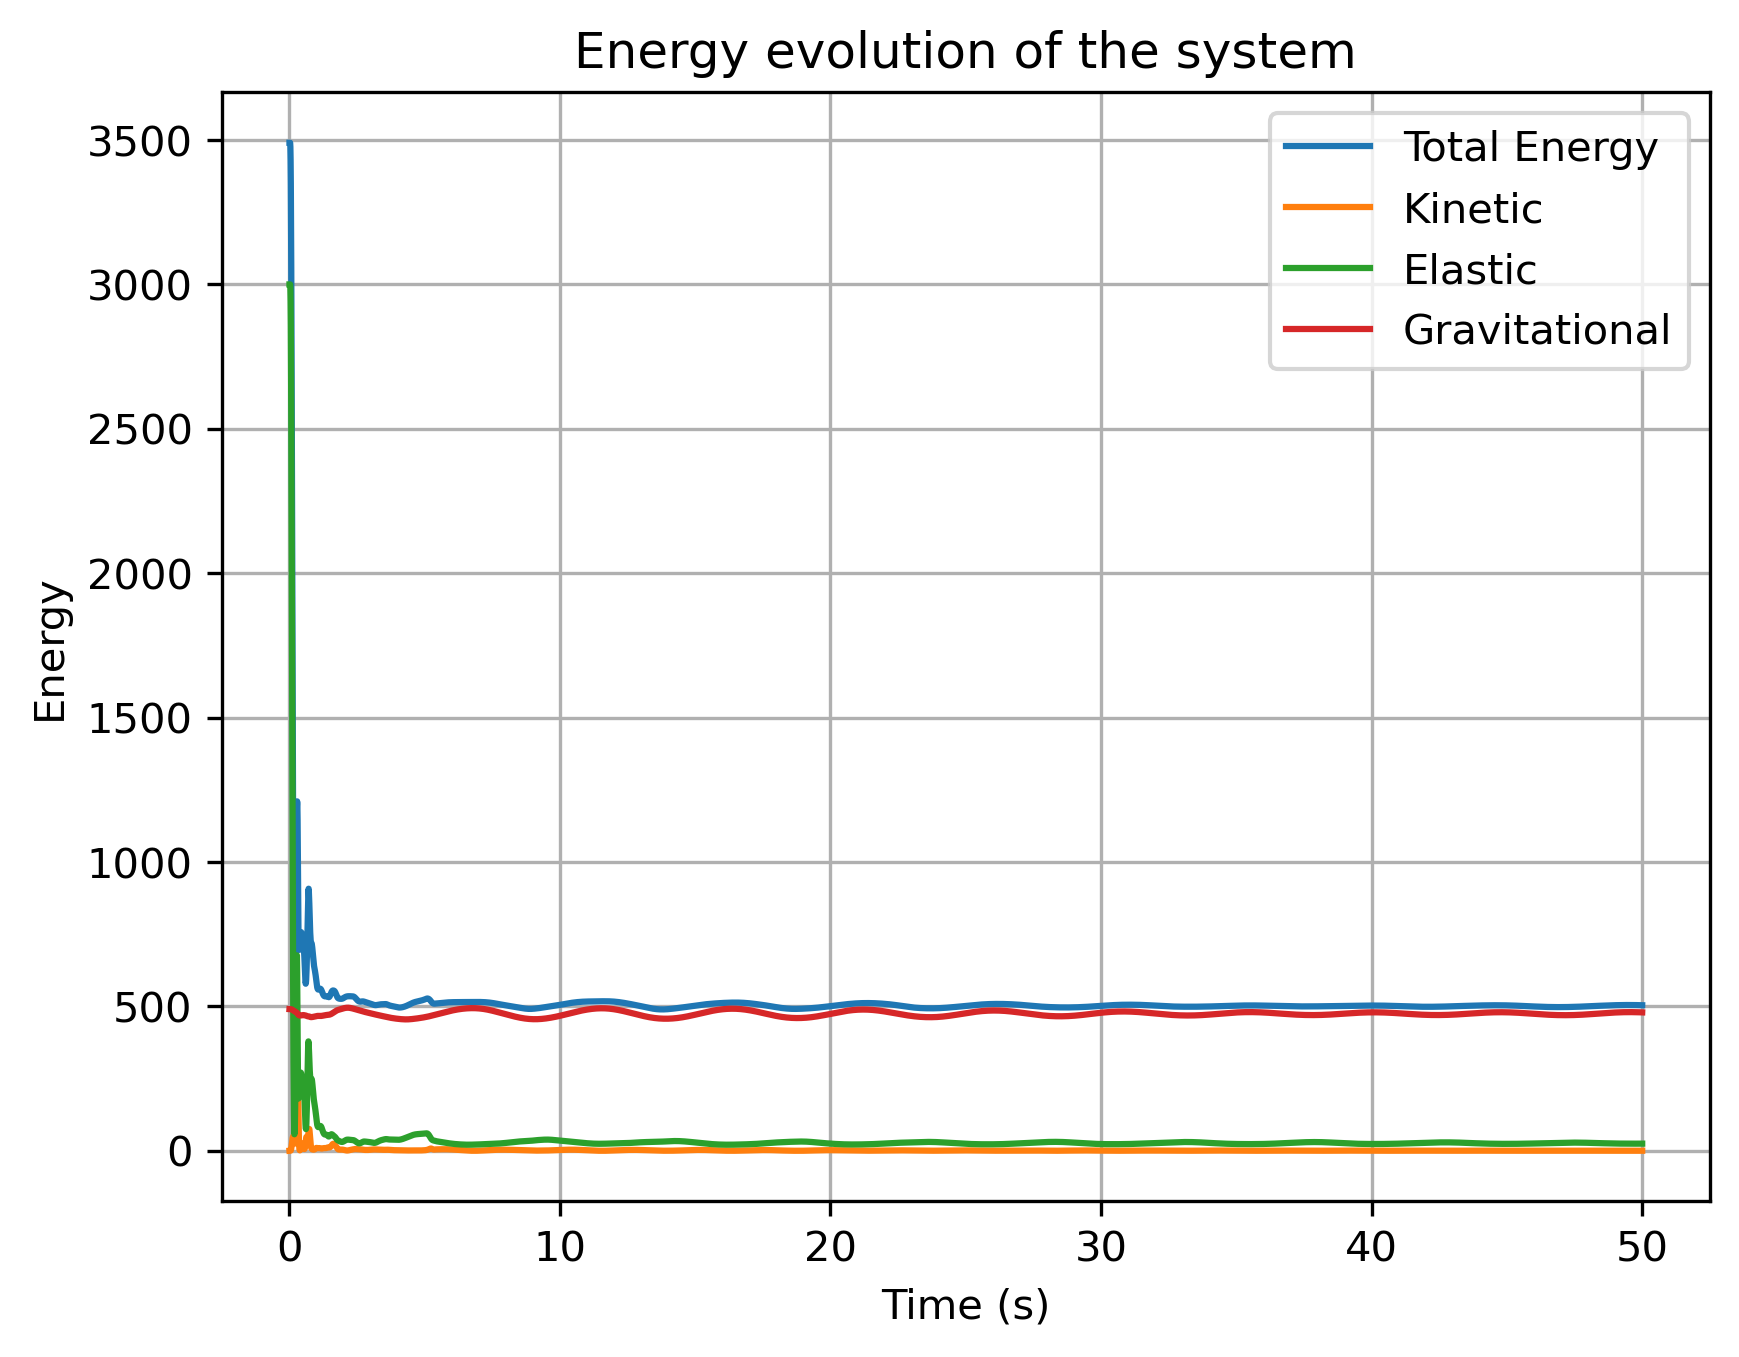
\includegraphics[width=\linewidth]{simulation_data_len1_k400_energy_50s}
    \caption{First 50 seconds (Repeat of \ref{fig:pos_k400_s}.b}
\end{subfigure}
\hfill
\begin{subfigure}[b]{0.48\linewidth}
    \centering
    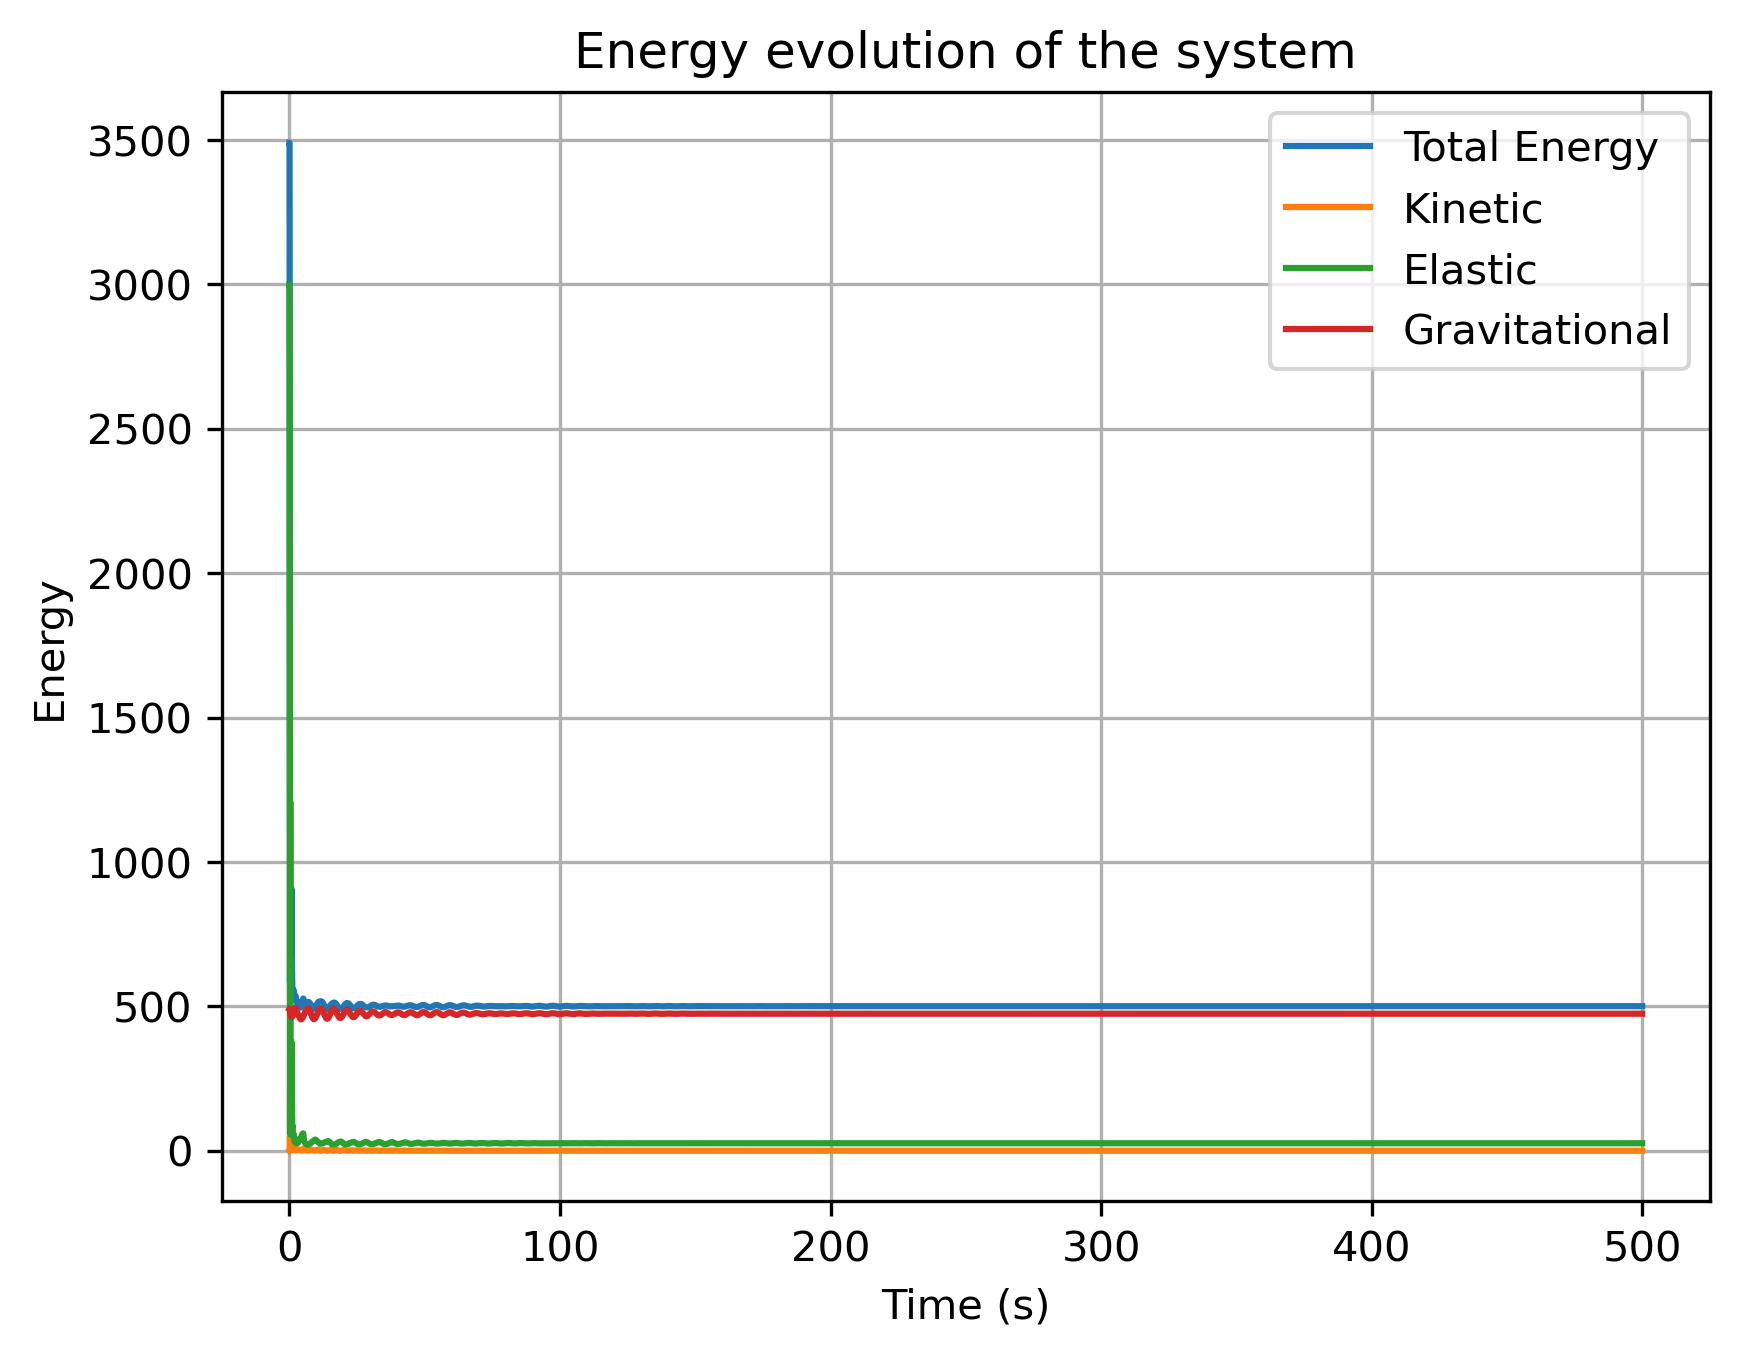
\includegraphics[width=\linewidth]{simulation_data_len1_k400_energy_500s}
    \caption{First 500 seconds}
\end{subfigure}
\caption{Energy evolution for spring stiffness $k=400$ with damping $c=k/20$. The stiffer system exhibits even faster oscilations, converging to equilibrium.}
\label{fig:energy_k400_l}
\end{figure}

\begin{figure}[H]
\centering
\begin{subfigure}[b]{0.48\linewidth}
    \centering
    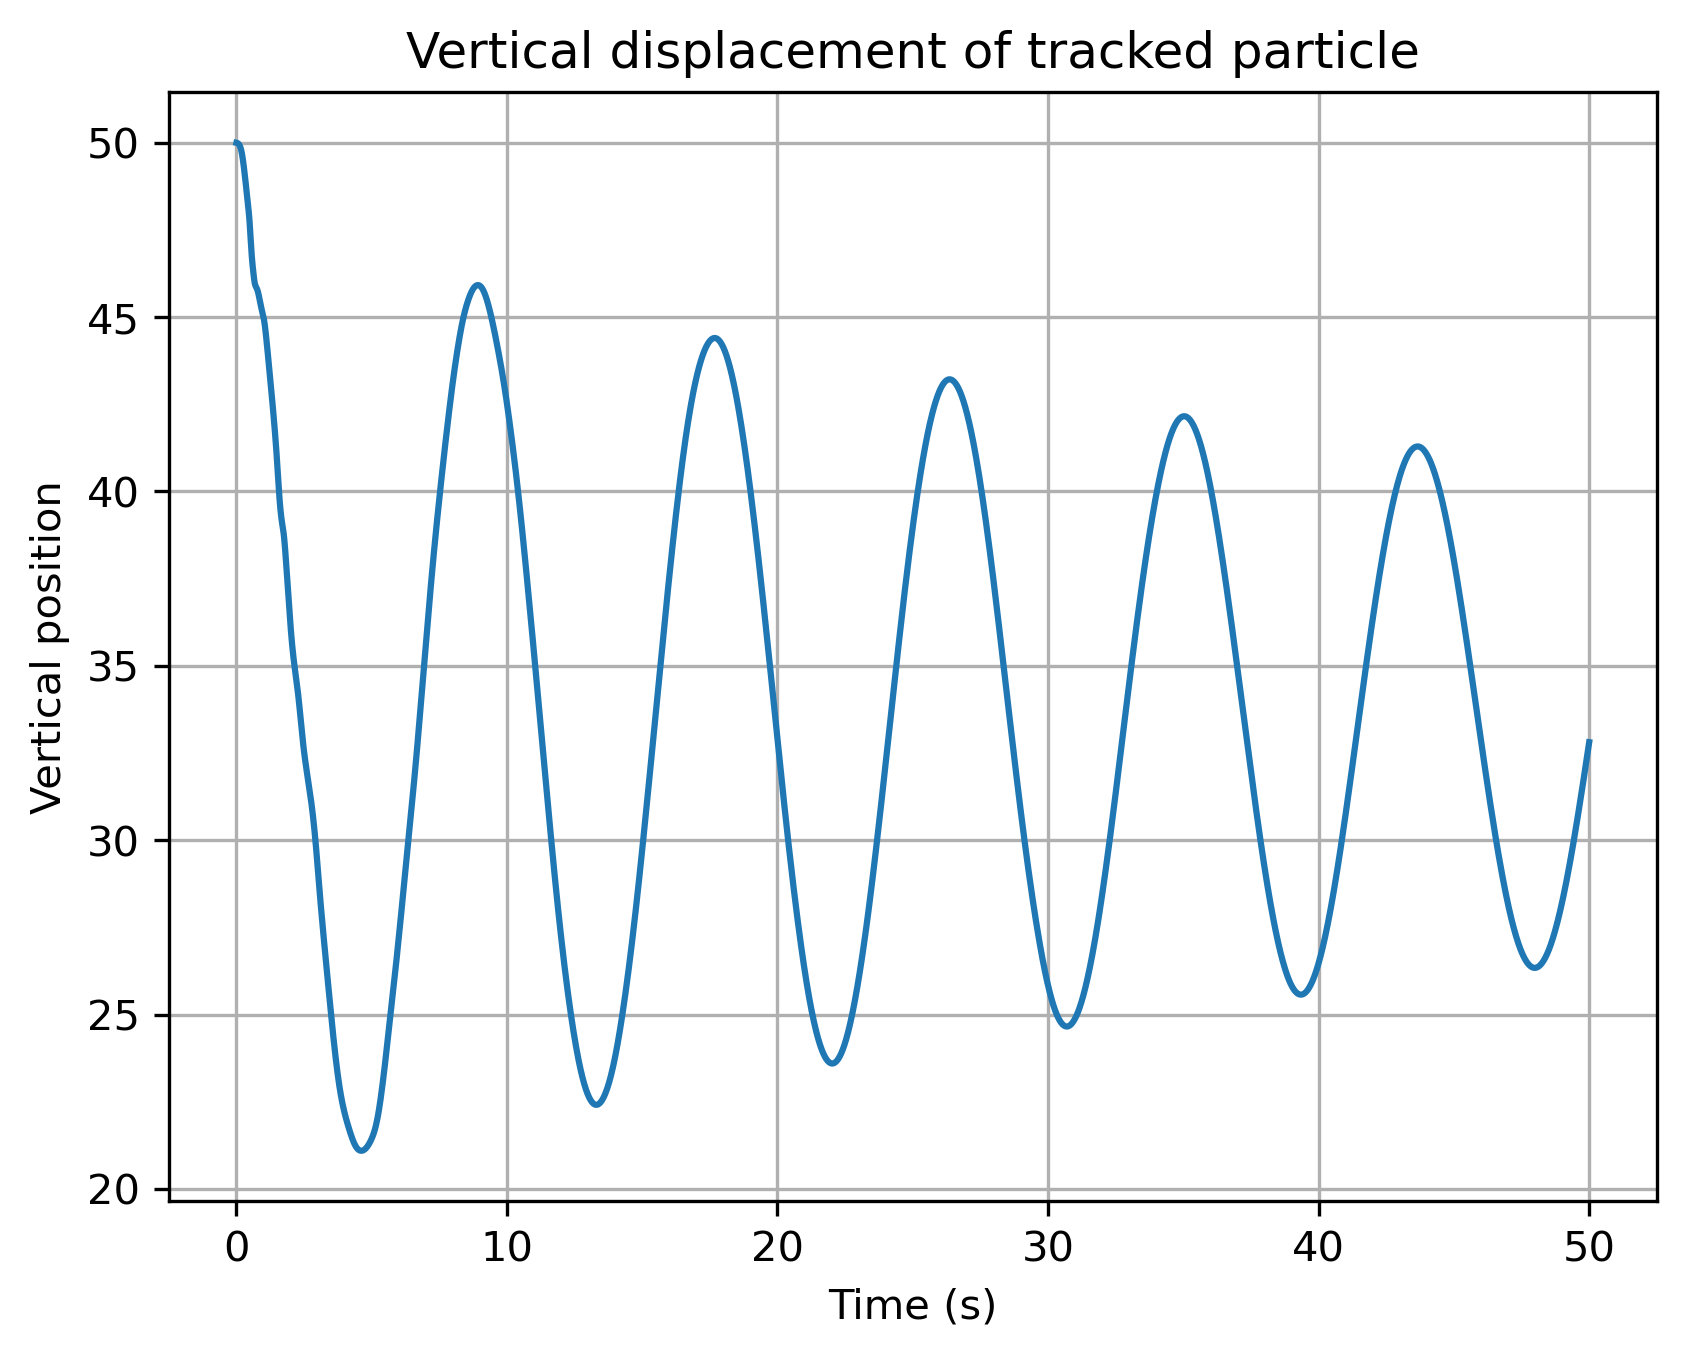
\includegraphics[width=\linewidth]{simulation_data_len1_k100_pos_50s}
    \caption{First 50 seconds}
\end{subfigure}
\hfill
\begin{subfigure}[b]{0.48\linewidth}
    \centering
    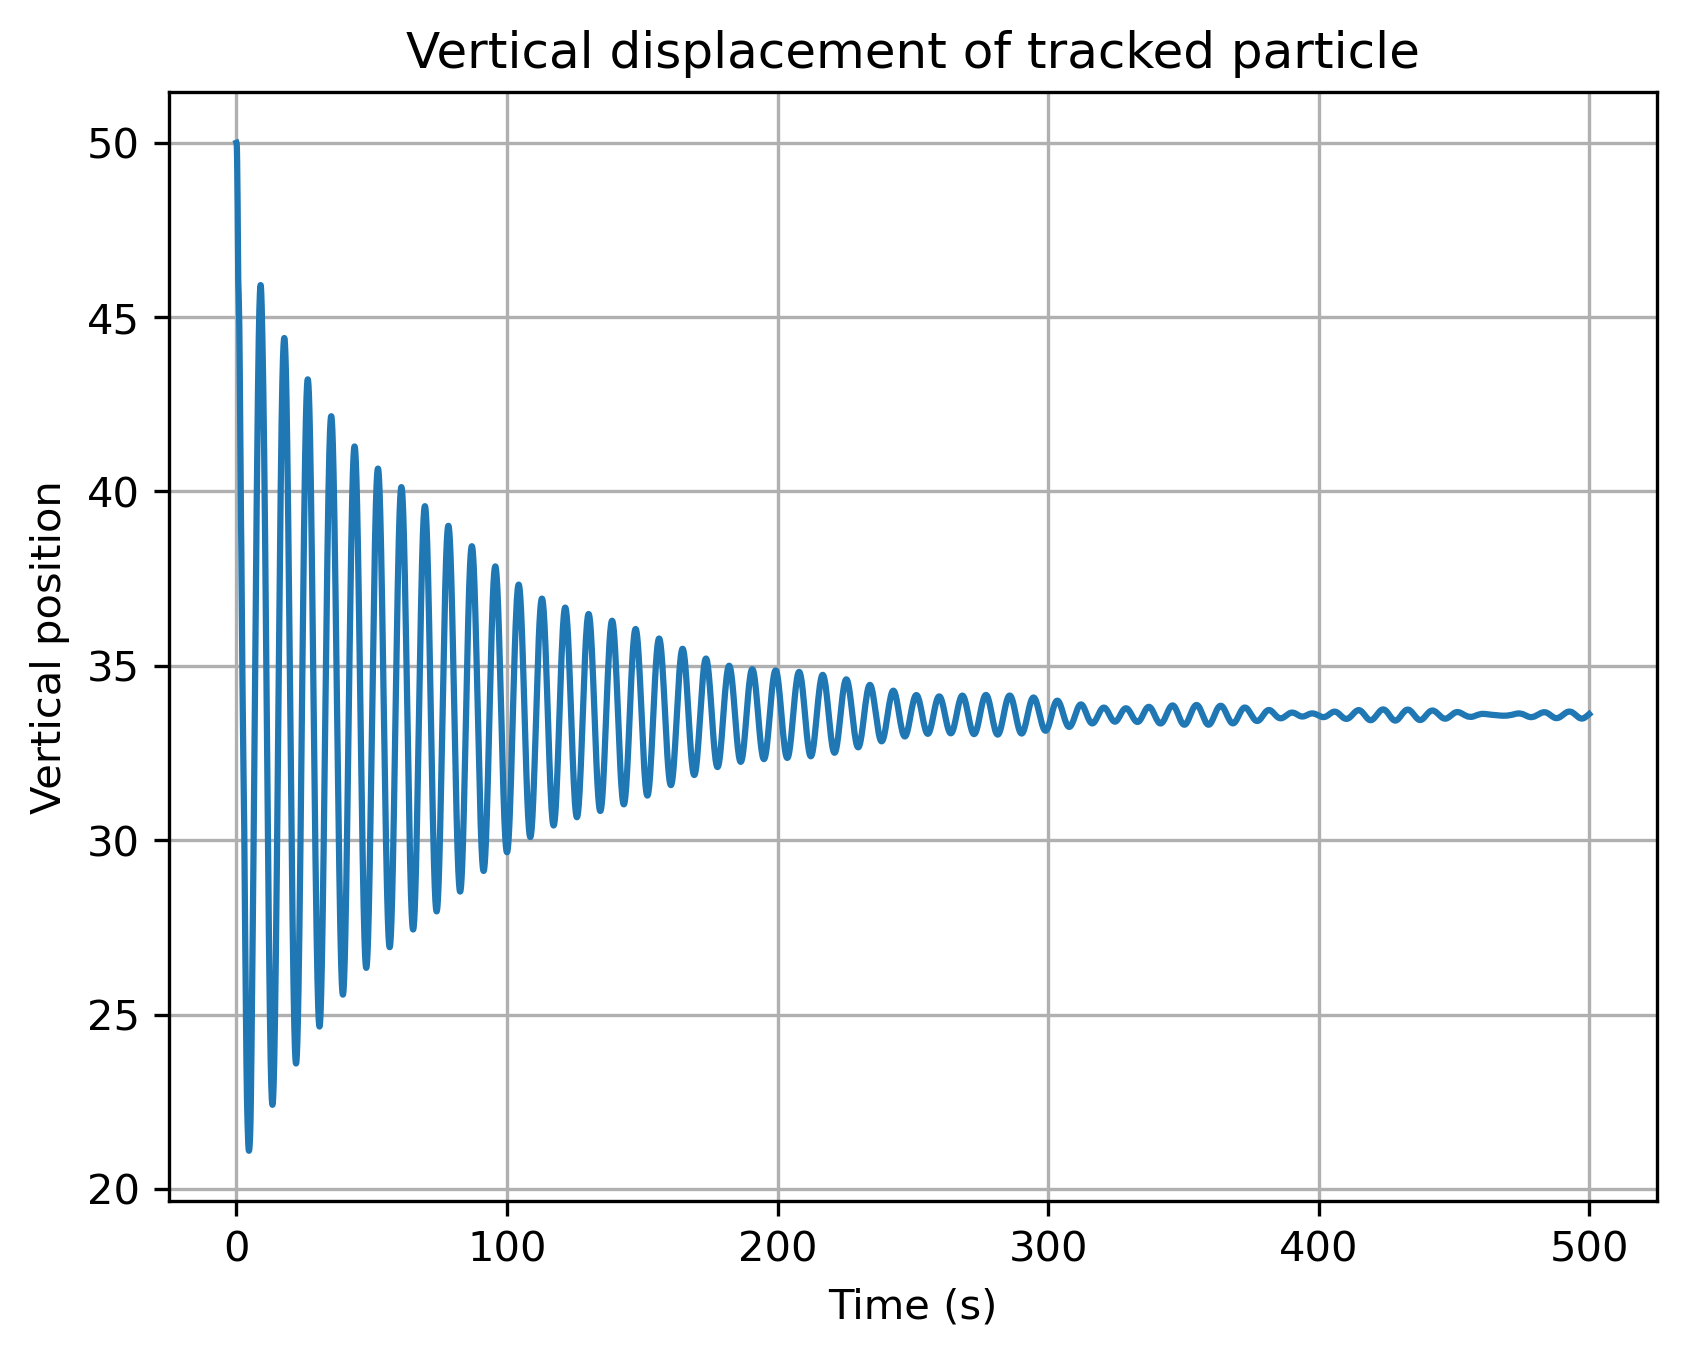
\includegraphics[width=\linewidth]{simulation_data_len1_k100_pos_500s}
    \caption{First 500 seconds}
\end{subfigure}
\caption{Position displacement for spring stiffness $k=100$ with damping $c=k/20$.}
\label{fig:pos_k100}
\end{figure}

\begin{figure}[H]
\centering
\begin{subfigure}[b]{0.48\linewidth}
    \centering
    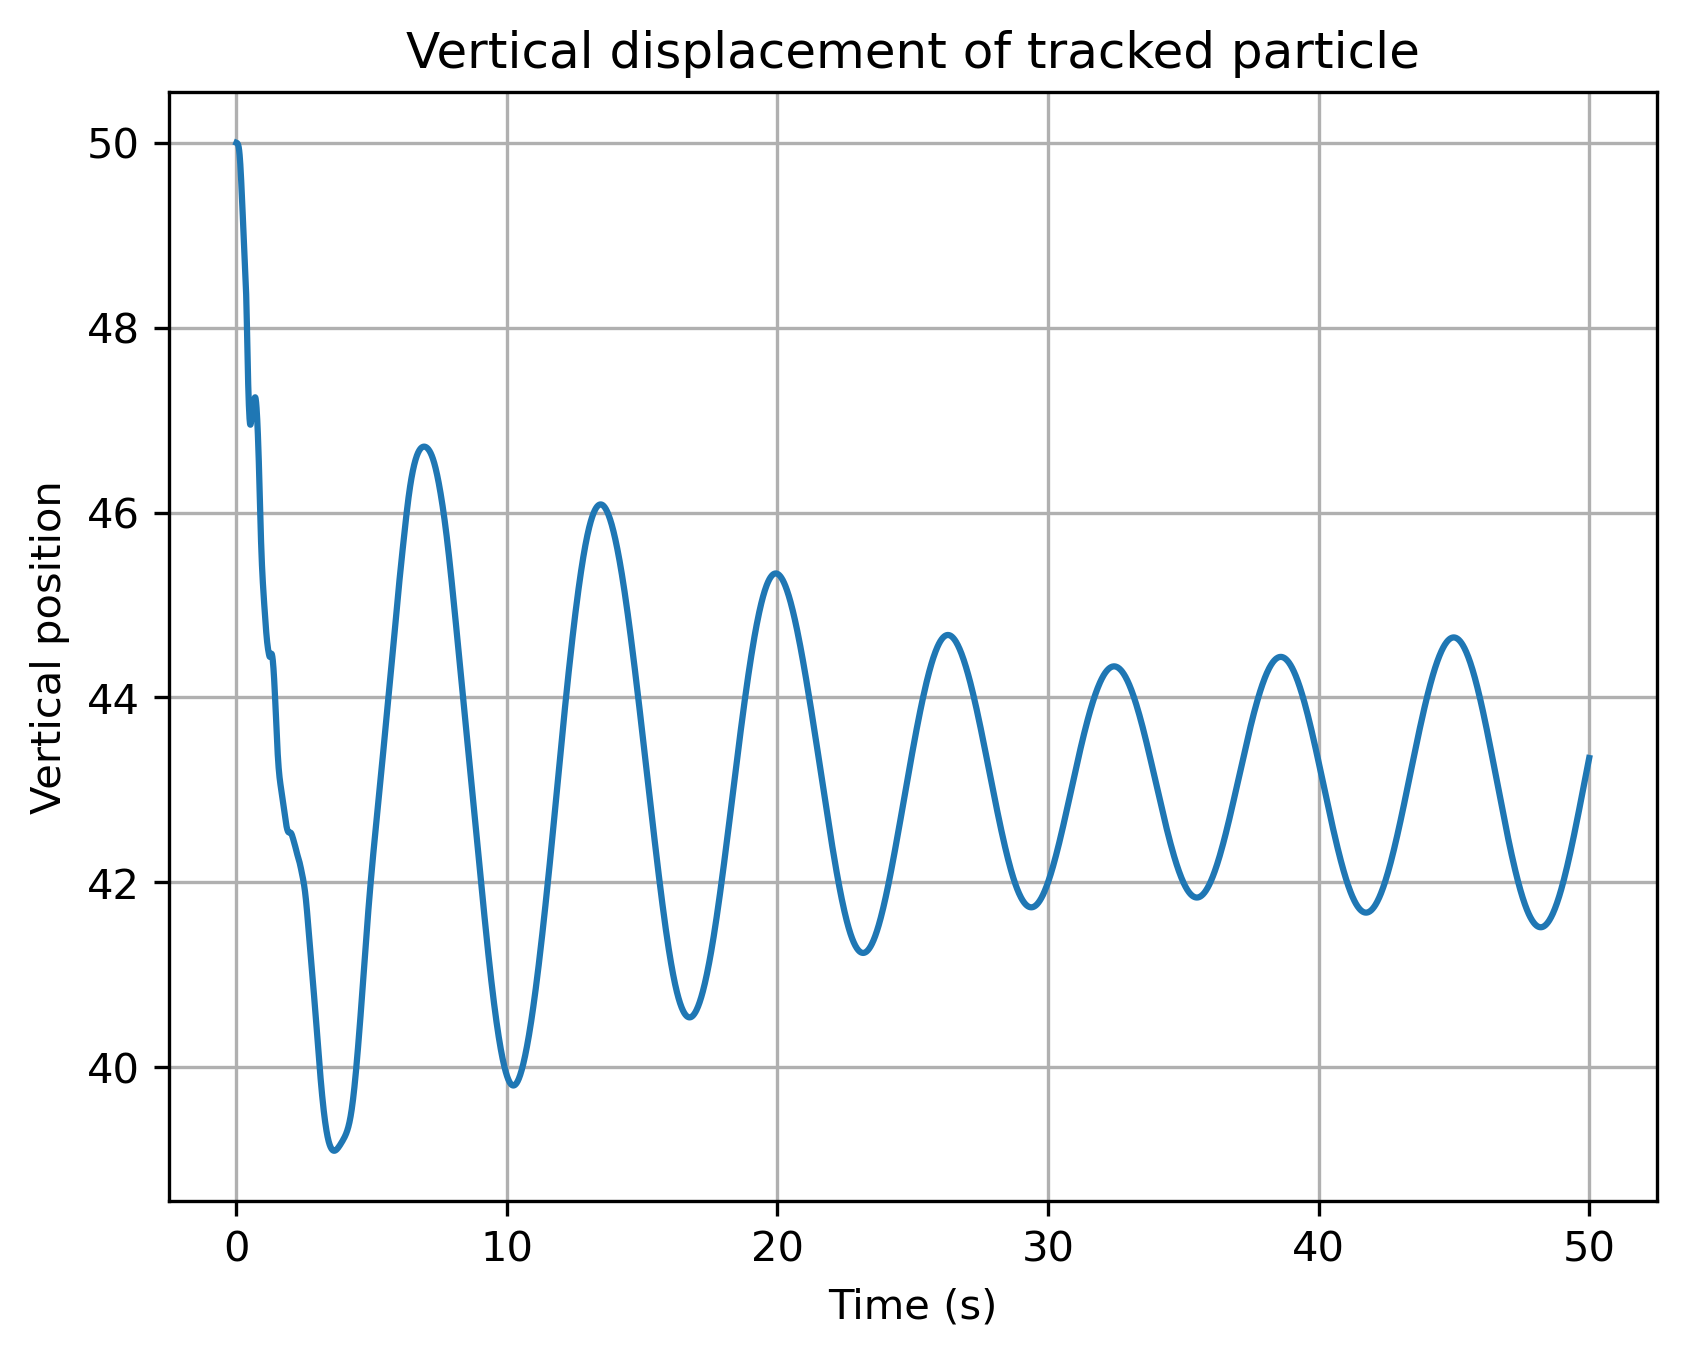
\includegraphics[width=\linewidth]{simulation_data_len1_k200_pos_50s.png}
    \caption{First 50 seconds}
\end{subfigure}
\hfill
\begin{subfigure}[b]{0.48\linewidth}
    \centering
    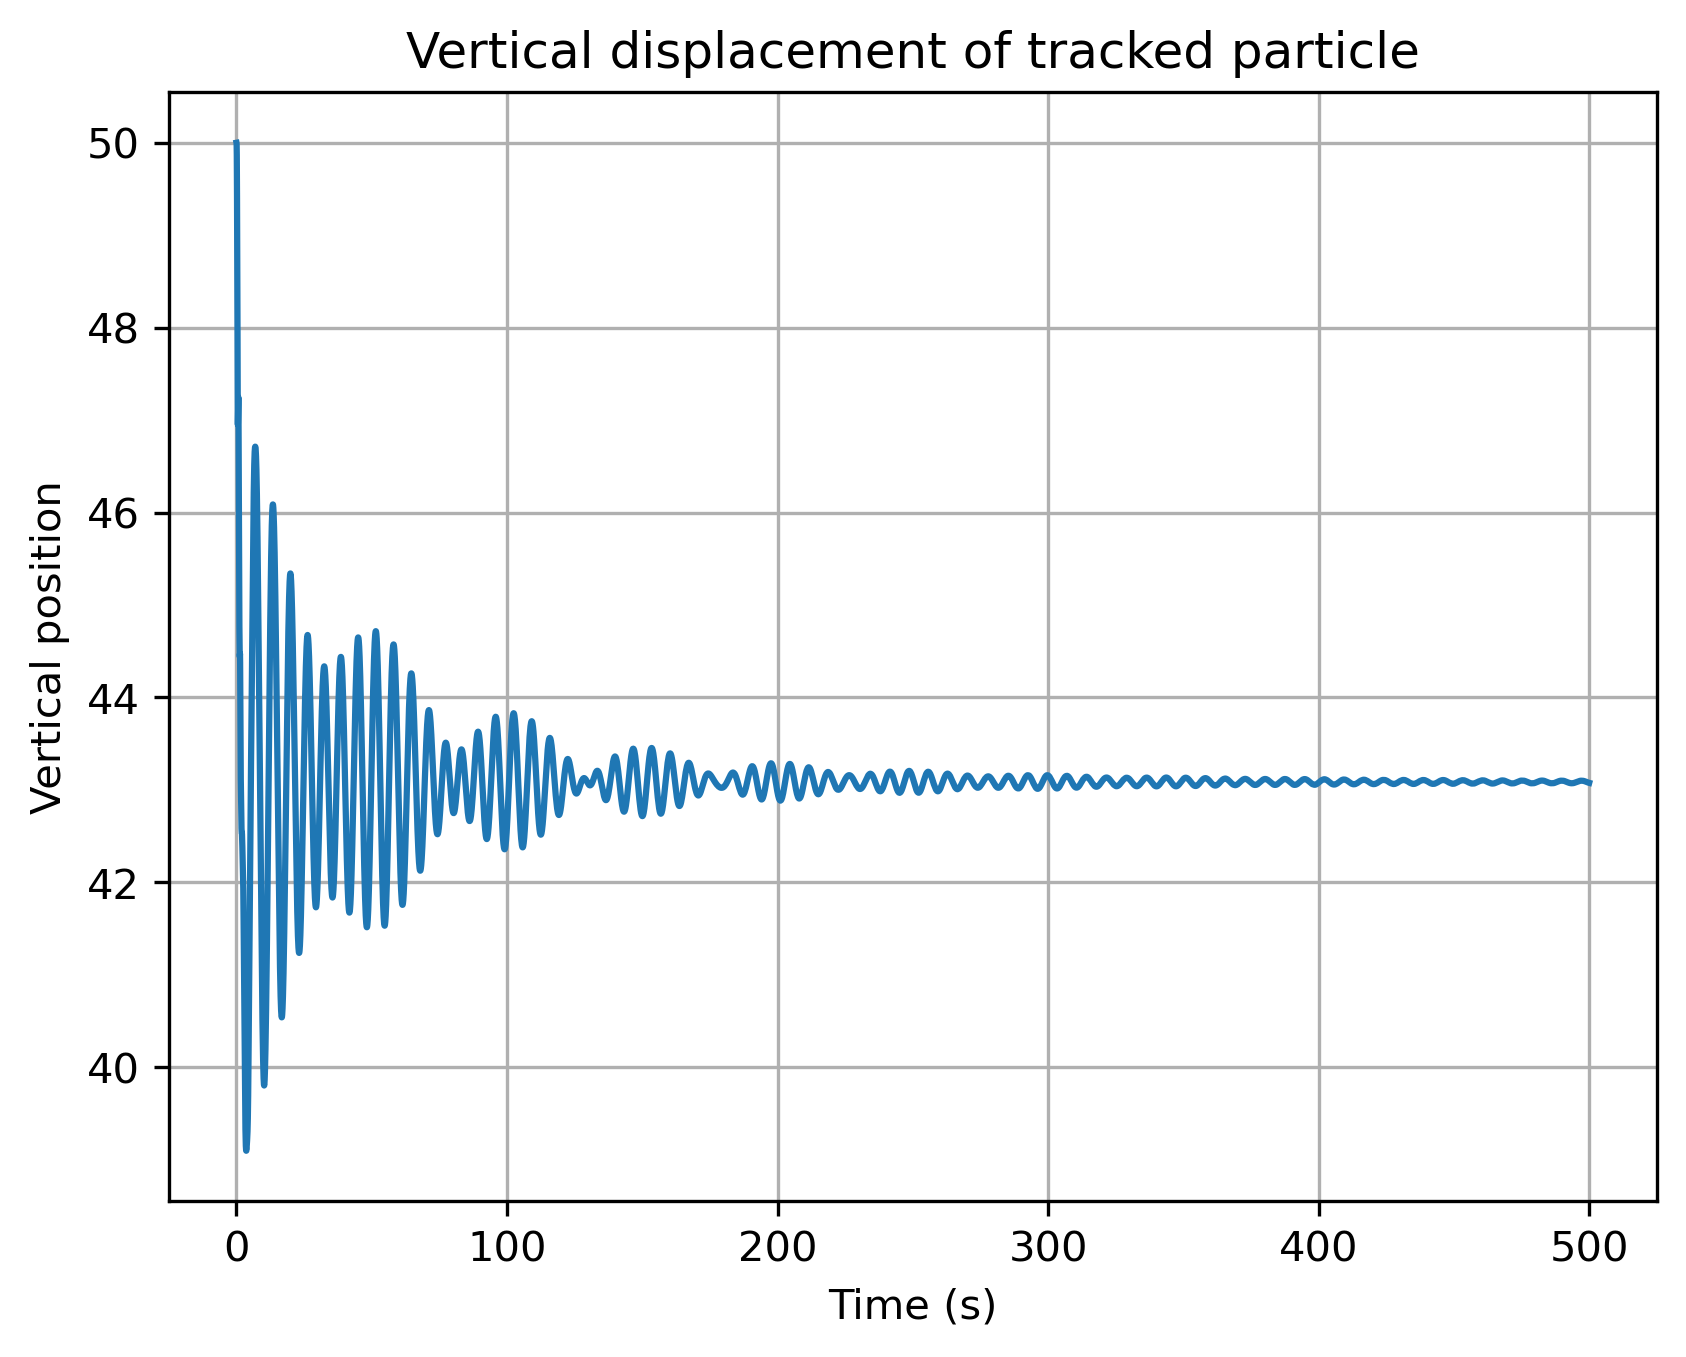
\includegraphics[width=\linewidth]{simulation_data_len1_k200_pos_500s}
    \caption{First 500 seconds}
\end{subfigure}
\caption{Position displacement for spring stiffness $k=200$ with damping $c=k/20$. Increased stiffness results in faster oscillations and stabilization to equilibrium.}
\label{fig:pos_k200}
\end{figure}

\begin{figure}[H]
\centering
\begin{subfigure}[b]{0.48\linewidth}
    \centering
    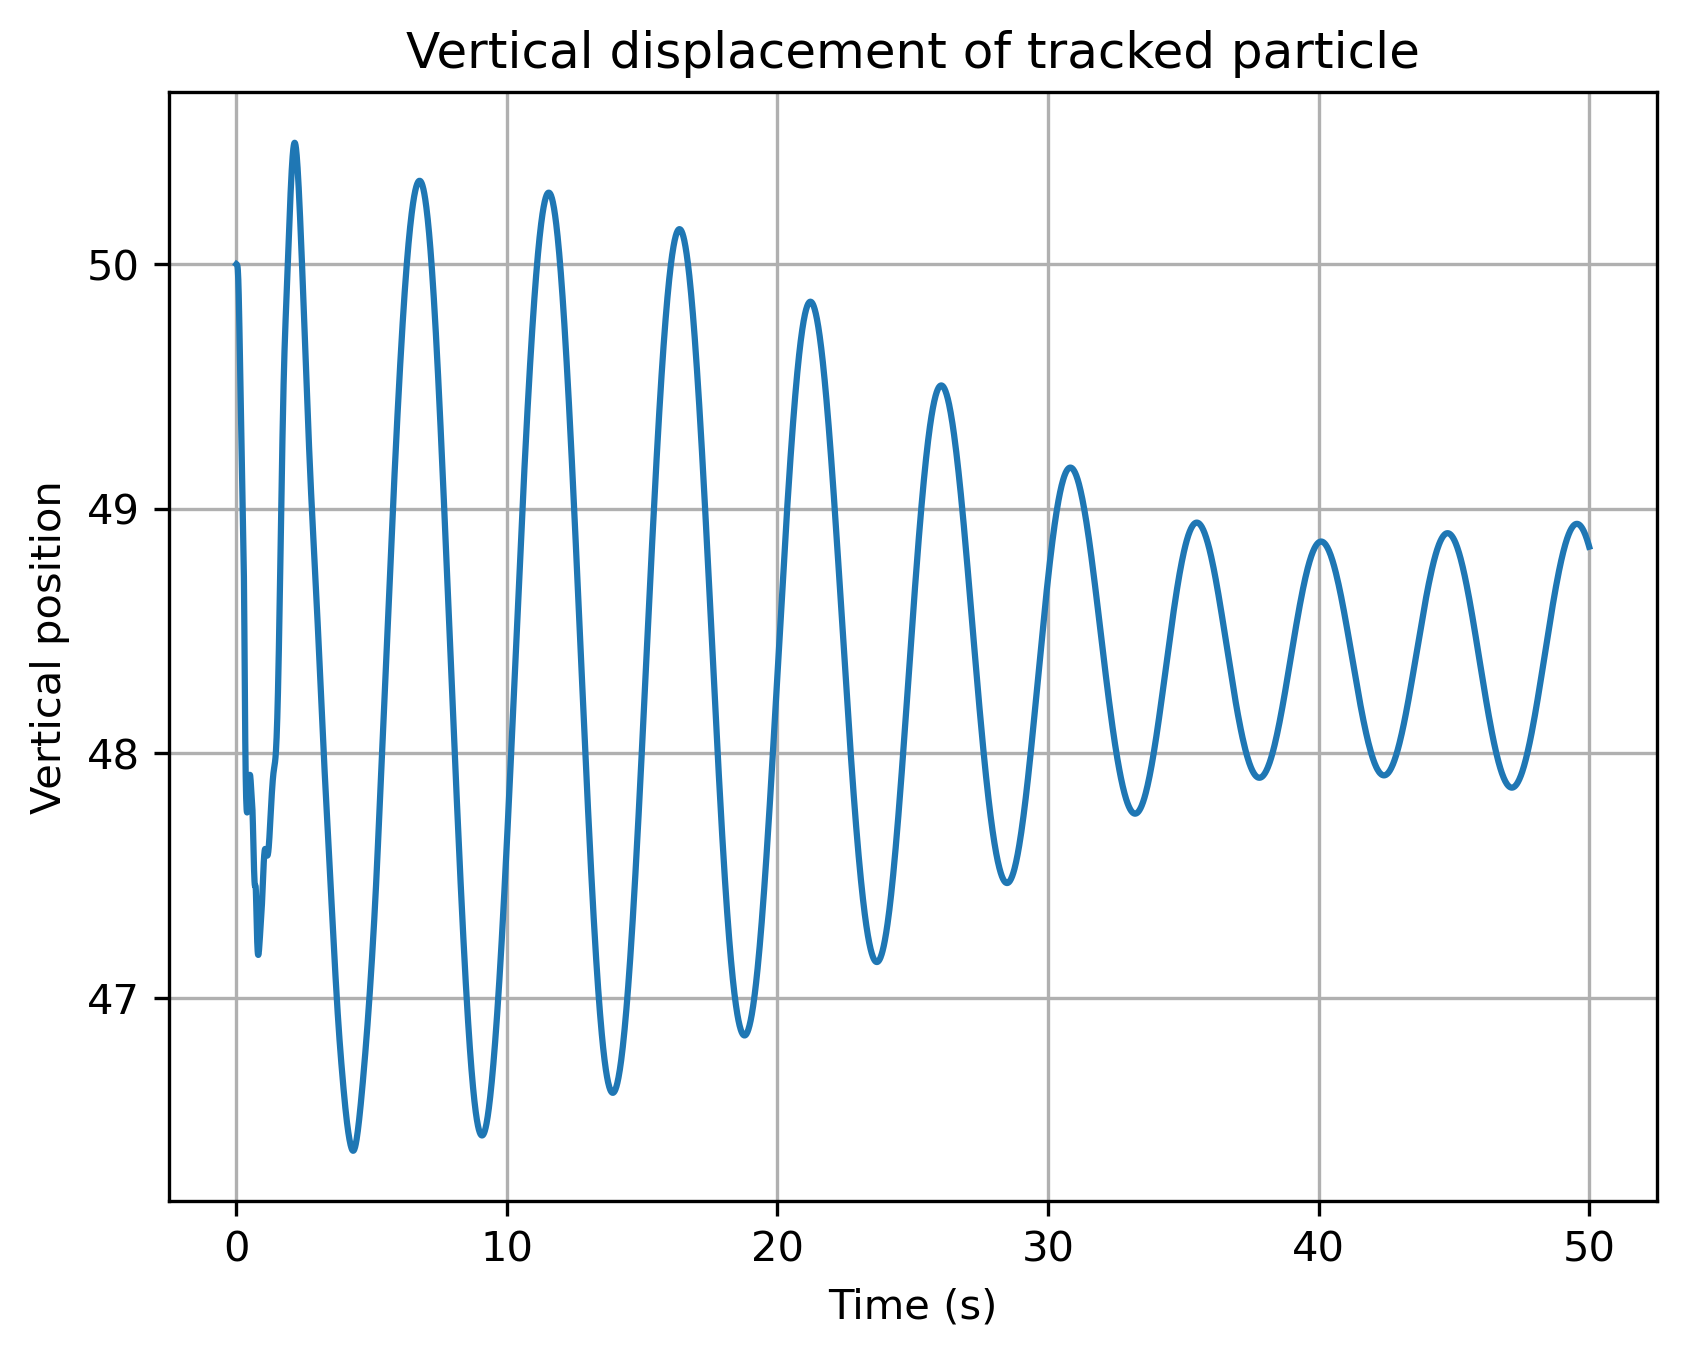
\includegraphics[width=\linewidth]{simulation_data_len1_k400_pos_50s}
    \caption{First 50 seconds}
\end{subfigure}
\hfill
\begin{subfigure}[b]{0.48\linewidth}
    \centering
    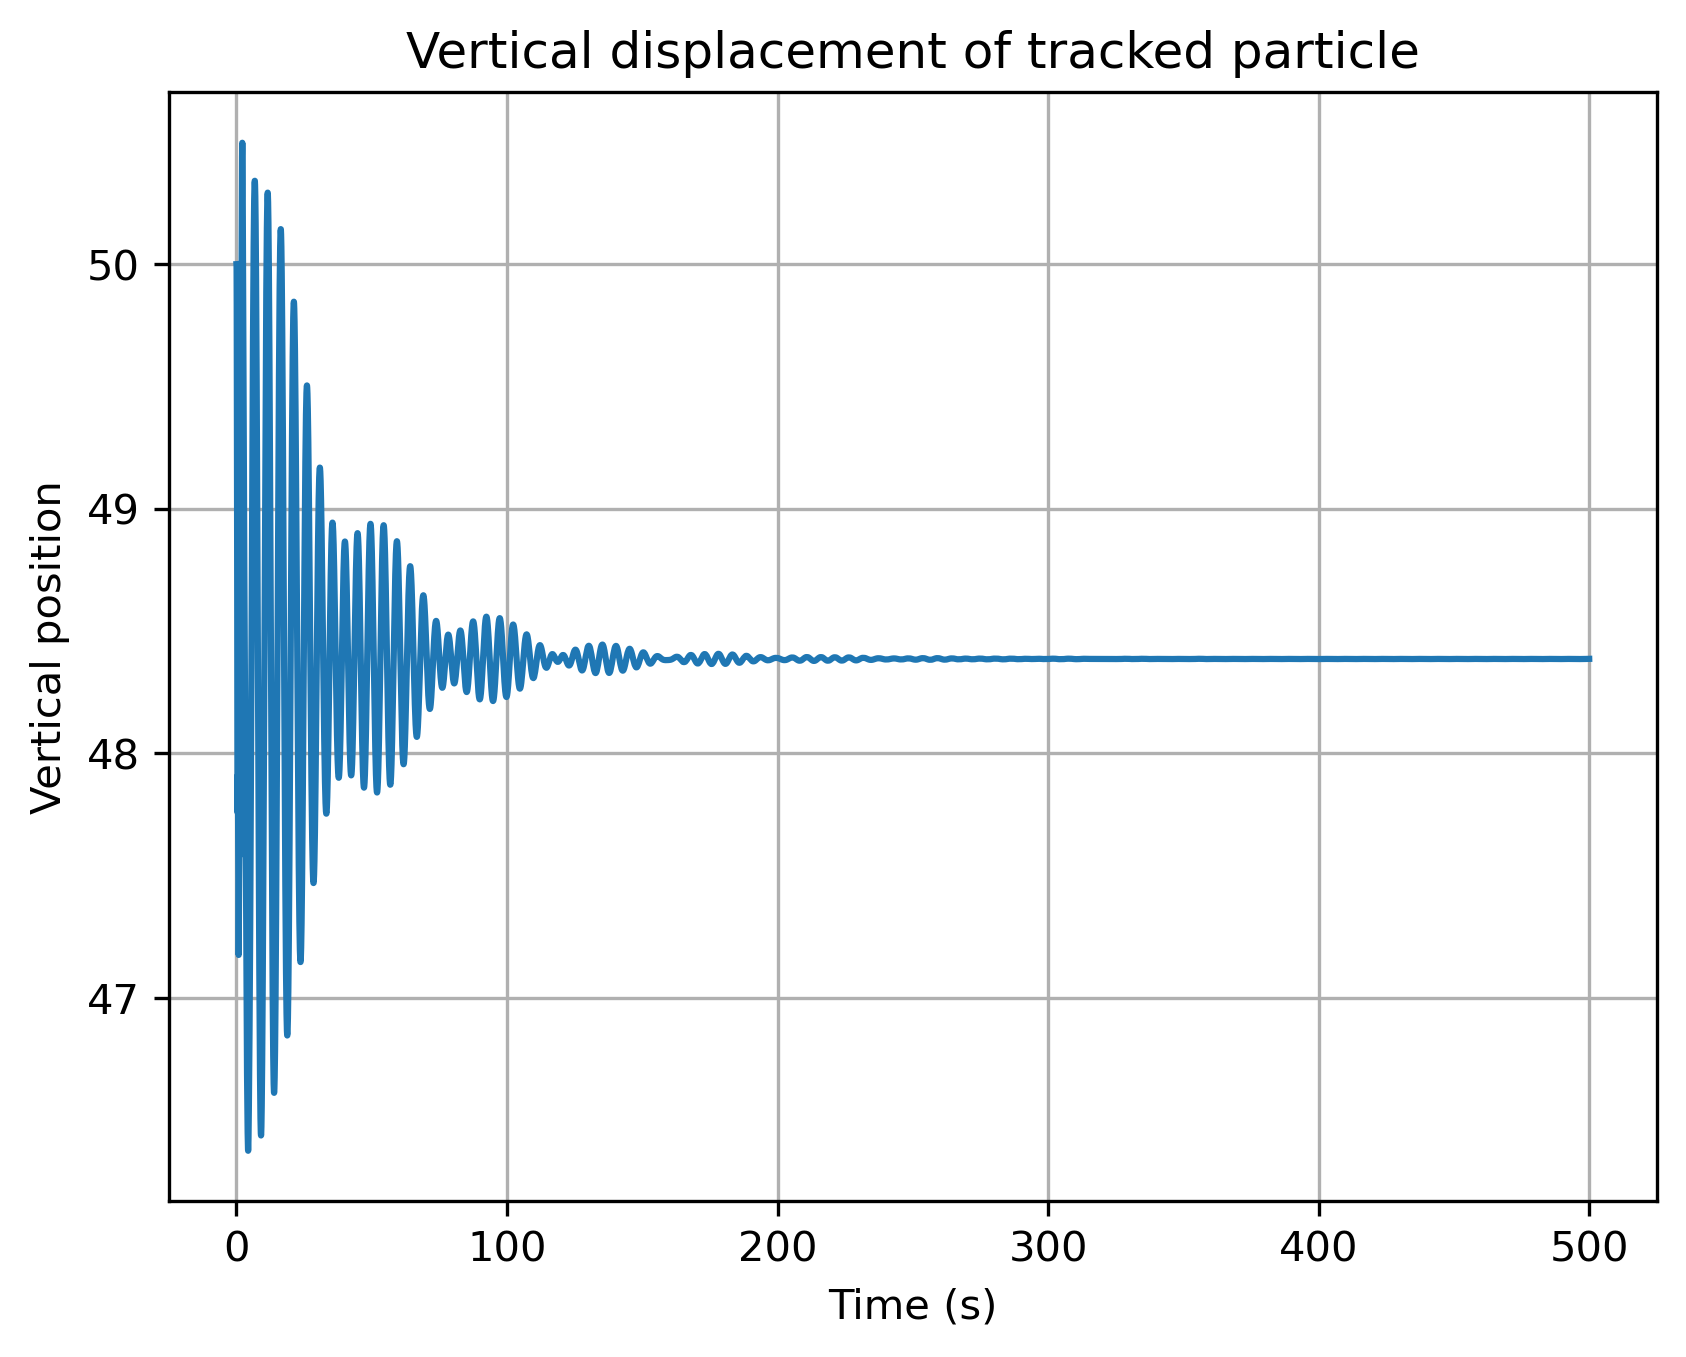
\includegraphics[width=\linewidth]{simulation_data_len1_k400_pos_500s}
    \caption{First 500 seconds}
\end{subfigure}
\caption{Position displacement for spring stiffness $k=400$ with damping $c=k/20$. The stiffer system exhibits very fast stabilization to equilibrium.}
\label{fig:pos_k400}
\end{figure}

When the simulation is extended to $500$ seconds (Figures~\ref{fig:energy_k100_l}--\ref{fig:energy_k400_l} and corresponding position plots), the system exhibits a notable long-term behavior: after the initial transient decay, the system settles into a low-amplitude oscillatory behavior that decays towards equilibrium.

Both the energy plots and the vertical displacement plots reveal the presence of two superimposed oscillatory modes:
\begin{itemize}
    \item A higher-frequency oscillation associated with local spring vibrations,
    \item A lower-frequency oscillation associated with global motion of the mass-spring structure under gravity and boundary constraints.
\end{itemize}

This dual harmonic behavior arises from the coupling between internal elastic modes and the global gravitational potential as energy continues to exchange between the two terms. The viscous damping reduces the initial high-energy oscillations, and decays the oscillations until the system approaches a static rest state.

\subsection{Effect of Spring Stiffness}
\label{Sec7.5:StiffnessEffect}

Comparing results across different stiffness values reveals clear quantitative trends. Increasing the spring stiffness leads to higher peak elastic energy during the initial transient phase, as stiffer springs resist deformation more strongly. This effect is visible in the elastic energy curves for $k = 200$ and $k = 400$, which reach higher maxima than those for $k = 100$.

Because physically, the damping coefficient required to overcome the effect of the elastic energy does not scale linearly with the stiffness, the behavior modeled by the system shows a different rate of energy dissipation for each value of stiffness. The higher damping coefficient of higher stiffness tests result in faster decay towards equilibrium despite having higher energy in the system. This behavior is consistent with the theoretical relationship between stiffness and damping.

\subsection{Comparison with Theoretical Models}
\label{Sec7.6:TheoreticalComparison}

The observed numerical behavior closely matches the predictions of both the Newtonian and Lagrangian formulations. The rapid conversion of elastic potential energy into kinetic energy is consistent with the force-based spring model and the energy-gradient interpretation of the Lagrangian approach. Likewise, the monotonic decay of total mechanical energy confirms the presence of dissipative forces modeled through the Rayleigh dissipation function.

The equivalence between the Newtonian and Lagrangian equations of motion is further supported by the consistent qualitative behavior across all stiffness values. Although the integration scheme is explicit and the system is highly nonlinear, the simulation preserves expected physical trends such as energy dissipation, oscillatory motion, and convergence to equilibrium.

Overall, the results demonstrate that the implemented mass-spring-damper model faithfully reproduces the physical behavior predicted by classical mechanics, validating both the theoretical derivations and the numerical implementation.

\subsection{Limitations}
\label{Sec7.7:Limitations}

Although the mass-spring model captures many qualitative features of elastic behavior, it does not enforce strict volume preservation or prevent large shear deformations. As a result, the simulated material should be interpreted as an approximate elastic medium rather than a physically exact solid. Nevertheless, for the purposes of demonstrating Newtonian and Lagrangian dynamics, the model provides a clear and effective framework.


% -------------------------------------------------
\section{Conclusion}
\label{Sec8:Conclusion}

This work presented the formulation, implementation, and analysis of a three-dimensional deformable body simulation based on a mass-spring-damper model. The governing equations of motion were derived using both Newtonian mechanics and Lagrangian dynamics with Rayleigh dissipation, demonstrating the equivalence between force-based and energy-based formulations for this class of systems. The resulting nonlinear, coupled equations were integrated numerically using a momentum-based semi-implicit scheme with substepping to ensure stability.

In the early stages, higher-frequency oscillations dominated due to strong local spring compression, while lower-frequency modes emerged as the structure relaxed globally. These combined effects produced a dual harmonic appearance in both the displacement and energy plots. Increasing spring stiffness resulted in larger initial elastic energy, higher oscillation frequencies, and longer decay times, despite damping being scaled proportionally to stiffness. This behavior highlights the competing effects of stiffness and damping in Rayleigh-damped systems: while increased damping accelerates energy dissipation locally, increased stiffness raises natural frequencies and stores more energy, prolonging the transient response. Nevertheless, in all cases, total mechanical energy decreased monotonically over long time horizons, confirming the dissipative nature of the model.

Overall, the simulation demonstrates that a mass--spring--damper system with Rayleigh dissipation provides a physically consistent and numerically tractable approximation of elastic body behavior. The agreement between theoretical predictions and measured results confirms the correctness of both the mathematical formulation and the implementation.

\nocite{*}
\bibliographystyle{plain}
\bibliography{citations}
\end{document}
